\documentclass{subfiles}

\begin{document}

    \chapter{Implementaciones sobre el sistema de Realidad Aumentada}
    \label{chap:3}

        \section{Modelo en 3D y Three.js}
        \label{sec:modelo_en_3d_y_three_js}
        A partir del sistema básico generado en el capítulo anterior, podemos empezar a añadirle complejidad a nuestro sistema. El primer elemento que añadiremos es un modelo en 3D que utilizaremos como base en esta aplicación.

        \paragraph{}
        Para la carga, inserción, control y movimientos de los modelos en 3D se ha utilizado en esta aplicación la librería \threejs. \threejs es una librería ligera preparada para su uso en aplicaciones web compatible con \js \cite{web:wikipediathreejs}. Además, este está especializado en el control de modelos en 3D en formato \glb y \gltf, que son dos formatos basados en \textit{JSON} y que están creados para ser óptimos en tiempo de ejecución (el formato \glb es el equivalente en binario a \gltf) \cite{web:threejs_loading3dmodels}.

        \paragraph{}
        La librería \threejs basa su funcionalidad en el uso de Escenas o \textit{Scenes}, el objeto que utiliza esta librería para almacenar y presentar sus modelos en 3D, la iluminación o focos de luz que los alumbrarán y las cámaras virtuales que observarán a estos mismos \cite{web:threejs_scene}. Aplicando un símil sencillo, la Escena de \threejs podría equivaler a una escena de cine, donde los actores equivaldrían a los modelos en 3D, los focos equivaldrían a la iluminación y las cámaras equivaldrían a las cámaras virtuales. Este último concepto es muy importante, debido a que afectará continuamente al renderizado de los modelos en 3D.

        \paragraph{}
        La cámara virtual es la que simula el punto de vista del espectador, ya sea en \ra, en \rv o en otras virtualizaciones que utilicen modelos en 3D como son las simulaciones, los videojuegos o las películas de animación \cite{web:mozilla_virtualcamera}. A alto nivel, una cámara virtual, además de la posición del espectador, definiría también lo que este va a poder observar de manera que, cuando se va a renderizar una imagen, solo tiene que generarse la parte visible de los modelos que entren en el rango de visión de la cámara virtual.

        \begin{figure}
        \centering
        \fbox{
        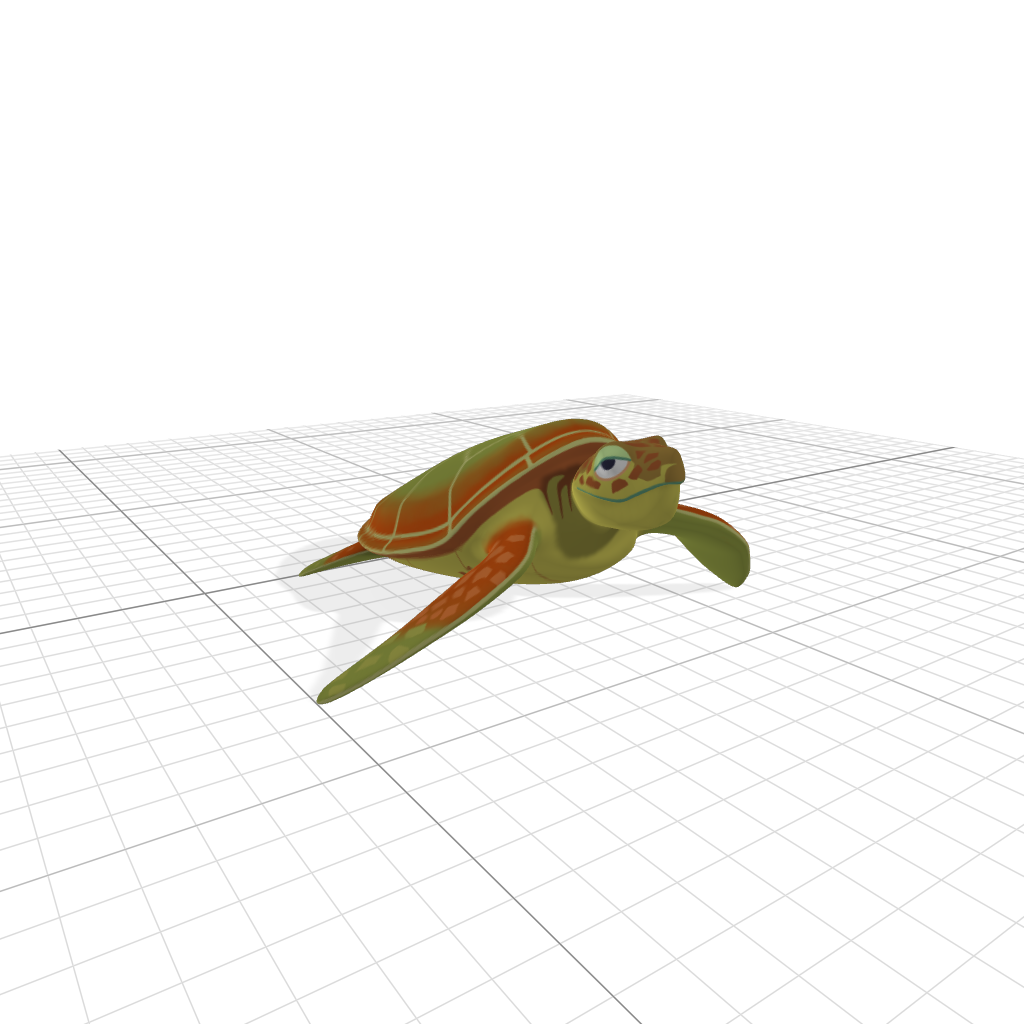
\includegraphics[width=0.6\textwidth]{img/tortuga_marina.png}
        }
        \caption{Ejemplo de renderizado de un modelo en 3D extraído de la biblioteca de modelos 3D de la aplicación de Windows \textit{Visor 3D}.}
        \label{fig:tortuga_marina}
        \end{figure}

        \paragraph{}
        Visualizando esto último con un ejemplo, en la figura \ref{fig:tortuga_marina} se ha renderizado un modelo 3D de una tortuga marina. En este renderizado, la cámara virtual se encuentra frente al modelo, pero ligeramente ladeado hacia la parte derecha de la tortuga. Debido a la posición de la cámara, no es necesario que se renderice la pata izquierda trasera de la figura, puesto que lo tapa el resto del cuerpo. Sin embargo, si la cámara se encontrase detrás de la tortuga, sería necesario renderizar ambas patas traseras y la cola, pero no se renderizaría la cara de la figura. De la misma manera, si la cámara no estuviese apuntando hacia la tortuga, no habría ningún modelo 3D que renderizar.
        
        \paragraph{}
        Aunque este parezca un concepto obvio, es necesario explicarlo, debido a que será necesario establecer la posición y orientación de la cámara virtual durante el desarrollo. Esto es porque la cámara virtual coincidirá con la posición de la cámara del dispositivo móvil. Cuando la cámara apunte hacia una figura en 3D en la \ra, se incrustará en la pantalla del móvil la parte de la figura que se vea desde la cámara virtual (es decir, se debe ver por la pantalla lo que se vería a través de la cámara si esta figura existiese en nuestra Realidad).

        \paragraph{}
        Una vez explicado esto, es necesario volver al código. Siguiendo el orden de carga, el primer lugar donde nos detendremos es en la función \textit{callback} \textit{checkSessionSupported}, vista en la sección \ref{sec:sesion_webxr}, que es la función que se lanza desde el constructor del Controlador y que inicializaba los elementos más pesados antes de que el usuario pulsase el botón de iniciar la Sesión de \ra. En esta, ya habíamos visto las acciones que se realizaban en caso de que el navegador no fuese compatible con \webxr, pero ahora vamos a ver algunas de las que se ejecutan en el caso positivo. Ampliando el código \ref{lst:2.2} al que hacemos mención:

\newpage
\begin{lstlisting}[language=JavaScript, caption={Carga de elementos de Three.js si se soporta la sesión.}, label={lst:3.1}]
// Constantes
#RETICLELINK = "http://url_donde_se_aloja_el_modelo_3d";

#checkSessionSupported = (isSupported) => {
    if (isSupported) {
    
        // Scene y Loader
        this.#scene = new THREE.Scene();
        this.#loader = new THREE.GLTFLoader();
        // ...

        // Modelo en 3D: Reticula
        this.#loader.load(this.#RETICLELINK, function(gltf) {
            // Figura
            this.#reticle = gltf.scene;
            this.#reticle.visible = false;
            this.#scene.add(this.#reticle);
        }.bind(this));
        // ...
    
    } else {
    
        document.getElementById("arButton").disabled = true;
        alert("Tu navegador no permite una sesi\xF3n de Realidad Aumentada.");
        
    }
};
\end{lstlisting}

        Aquí ya podemos ver tres elementos de cierto peso que se están cargando previamente antes de iniciar la Sesión: la Escena, una instancia de \textit{GLTFLoader} y, desde una función de esta última, un modelo 3D al que llamaremos a partir de ahora, <<retícula>>, sencillamente porque es el nombre del modelo original alojado en la librería de modelos de ejemplo de \webxr en GitHub. Este modelo en 3D, que podemos ver en la figura \ref{fig:reticle} será el que utilicemos como base para el funcionamiento de esta aplicación, haciendo las veces de <<puntero>> más adelante, cuando queramos señalar un punto en el suelo para ubicar el avatar que desarrollemos.

        \begin{figure}
        \centering
        \fbox{
        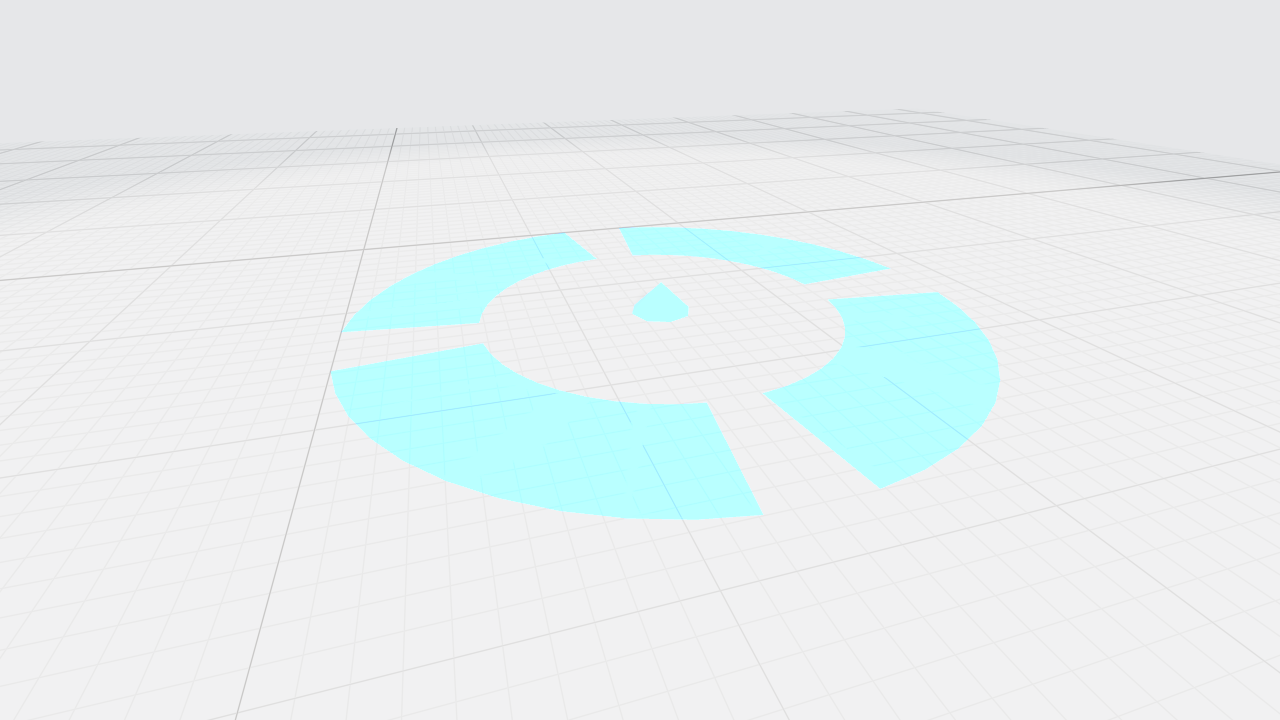
\includegraphics[width=0.6\textwidth]{img/reticle.png}
        }
        \caption{Muestra de la retícula utilizada en esta aplicación. Modelo obtenido del repositorio \textit{webxr} del perfil de \textit{Immersive Web at W3C}, en GitHub.}
        \label{fig:reticle}
        \end{figure}

        \paragraph{}
        En primer lugar, inicializamos la Escena en la línea 8 para poder introducir la retícula más adelante (volviendo al símil anteriormente utilizado, es como si el actor <<retícula>> entrara en escena). Sin embargo, esto no lo podemos hacer hasta que se haya cargado el modelo. Para esto, utilizamos el objeto \textit{GLTFLoader} de \threejs \cite{web:threejs_gltfloader}, que es inicializado en la línea 9 para poder ser usado a continuación. Este objeto contiene la función \textit{load()}, que permite cargar un modelo 3D (en este caso, en formato \gltf o \glb, dado que este objeto es una especialización del objeto \textit{Loader} y solo permite cargar archivos de dichos formatos) y lanzar una función \textit{callback} una vez obtiene un resultado. Mediante la función de \textit{GLTFLoader}, \threejs hace la traducción del contenido del fichero a objetos de \threejs que sean manejables desde código. Aunque la documentación no sea muy extensa sobre el objeto que ofrece esta función, sí se puede encontrar que, mediante la función \textit{callback} que creemos para esto, recibiremos un objeto (que en la línea 13 hemos llamado \textit{gltf}) que contiene los siguientes atributos \cite{web:discoverthreejs}:

        \begin{itemize}
            \item \textit{animations}: devuelve un array con las animaciones (\textit{THREE.AnimationClip}) que contenga el archivo con el modelo 3D. Estas animaciones, aunque ya entraremos más en detalle más adelante, no son más que conjuntos de posturas que, agrupados de la manera correcta, dan la sensación de movimiento si se van recorriendo a una velocidad adecuada.
            \item \textit{scene}: aunque el sistema llame al atributo también <<Escena>>, en verdad el objeto contenido es de tipo \textit{THREE.Group}. Este objeto se puede definir como un conjunto de mallas de triángulos, que son los que formarán las superficies de los objetos tridimensionales. Al recoger todas las mallas del archivo de manera unida como un solo grupo, estaremos recogiendo en verdad el modelo 3D al completo.
            \item \textit{cameras}: en caso de que el archivo contenga una cámara virtual preestablecida, podremos encontrarlo en este atributo, que nos devolverá un array de objetos \textit{THREE.camera}. Estas cámaras no nos servirán para la \ra, porque nosotros queremos solamente una cámara que se encuentre en todo momento en el punto de vista de la cámara del dispositivo móvil. Este atributo es mucho más útil cuando se pretende utilizar la librería para aplicaciones web de visualización de este tipo de figuras tridimensionales, como pueda ser \textit{Babylon.js Sandbox}.
        \end{itemize}

        Estos son los atributos más importantes, aunque también contiene otros que son de menor importancia para el desarrollo hasta ahora de este proyecto: 

        \begin{itemize}
            \item \textit{asset}: objeto de \js sin tipo (\textit{Object}) que contiene metadatos del archivo, comúnmente generados de forma automática por la herramienta de diseño utilizada para la construcción del modelo.
            \item \textit{parser}: objeto \textit{GLTFParser} que contiene la información del objeto que se ha utilizado internamente para transformar el archivo.
            \item \textit{scenes} (no confundir con \textit{scene}): de manera similar a \textit{scene}, contiene un array de objetos de tipo \textit{THREE.Group}. Esto se debe a que los archivos \gltf pueden contener varios grupos separados de mallas, aunque no será el caso en este proyecto.
            \item \textit{userData}: objeto sin tipado que contiene información customizada por parte del creador del archivo. Esta no está estandarizada, por lo que la información podría estar de cualquier manera.
        \end{itemize}

        Como se puede comprobar, son muchos los elementos que se cargan de un solo archivo, aparte del propio modelo en 3D. Esto se debe a que, como se verá más adelante, al diseñar un modelo en 3D se pueden añadir distintas propiedades preestablecidas. Más adelante, en la sección \ref{sec:animacion_de_modelos}, veremos como, desde el mismo archivo del modelo, podremos acceder también a las animaciones predefinidas que se encuentren contenidas en este. Sin embargo, durante este diseño también se pueden preestablecer otros elementos y guardarlos en el mismo archivo como iluminaciones y cámaras virtuales.

        \paragraph{}
        Una vez sabemos esto, y volviendo al código \ref{lst:3.1}, podemos ver que, en la línea 15, se está almacenando en el atributo privado \textit{reticle} del Controlador el grupo de mallas que formarán el modelo 3D de la retícula. Después de esto, se establece la propiedad \textit{visible} de este modelo a \textit{false} para hacerlo invisible hasta que nos interese, y se añade (esta vez sí) a la Escena de nuestra \ra. De esta manera, la figura se estará cargando desde un inicio para ser mostrada en cuanto esté preparada, teniendo en cuenta que todavía no se ha solicitado iniciar la Sesión de \ra.

        \paragraph{}
        En el momento en que el usuario pulse el botón, con estos elementos pesados ya cargados o, como mínimo, en proceso de ser totalmente cargados, se comenzará a preparar desde la función \textit{startLoop} el bucle de la función \textit{callback loopFunction}, donde también se cargarán algunos elementos de \threejs a mayores de los que vimos en los códigos \ref{lst:2.4} y \ref{lst:2.5} de la sección \ref{sec:procesado_iterativo}. Dado que este código puede quedar muy largo si se incluyen todos los elementos previamente vistos, todo lo que se haya explicado con anterioridad quedará resumido mediante un comentario de código:

\begin{lstlisting}[language=JavaScript, caption={Carga de elementos de Three.js antes de lanzar el bucle.}, label={lst:3.2}]
/** Opciones del renderizador de la RA. */
#RENDEREROPTIONS = {
    alpha: true
};

async startLoop() {
    // Carga de Canvas y GL
    // ...

    // Carga de Renderer
    this.#RENDEREROPTIONS.canvas = this.#canvas;
    this.#RENDEREROPTIONS.context = this.#gl;
    this.#renderer = new THREE.WebGLRenderer(this.#RENDEREROPTIONS);
    this.#renderer.autoClear = false;

    // Carga de Camera
    this.#camera = new THREE.PerspectiveCamera();
    this.#camera.matrixAutoUpdate = false;

    // Carga de Session
    // ...

    // Carga de Reference space
    this.#referenceSpace = await this.#session.requestReferenceSpace('local');

    // ...

    this.#session.requestAnimationFrame(this.#loopFunction);
}
\end{lstlisting}

        Dentro de esta función, podemos ver que se están preparando tres objetos distintos, de los cuales dos de ellos son parte de la librería \threejs. En primer lugar, se prepara el Renderizador, que es el objeto que se encargará de convertir el modelo 3D en imágenes que se insertarán en cada uno de los fotogramas que se muestren por pantalla \cite{web:threejs_webglrenderer}. Es muy importante tener en cuenta que el Renderizador superpondrá las imágenes de los modelos en 3D sobre las imágenes captadas por la cámara sin tener en cuenta el ángulo o la posición. Será trabajo del sistema que desarrollemos hacer que concuerde la posición del modelo con la superficie sobre la que se vaya a colocar. Para entender esto, es mejor ver las imágenes por separado:

        \begin{itemize}
            \item Primero, mediante \webxr, captaremos las imágenes de la cámara del dispositivo. \webxr también nos ofrecerá información que utilizaremos para calcular la pose en la que tendremos que colocar los modelos 3D. En el ejemplo de la figura \ref{fig:sample_ra_schema}, la imagen de la cámara correspondería con la fotografía de la izquierda.
            \item Después, mediante \threejs, colocaremos el modelo 3D en la posición adecuada usando la información del punto anterior. Además, también tendremos que colocar la cámara virtual de manera que apunte al modelo en el ángulo adecuado. En el ejemplo, la figura estaría colocada de tal forma que coincida la distancia entre la cámara virtual y la tortuga y la distancia entre el suelo y el dispositivo móvil. También coincidirá el ángulo de incidencia de ambas cámaras para que parezca que se observa desde el mismo sitio al mismo punto.
            \item Por último, se superpondrán las imágenes. Primero se colocará la imagen de la cámara sobre la pantalla, y nuestro sistema renderizará al modelo en la posición adecuada usando la librería \threejs para que nosotros superpongamos la imagen renderizada sobre la imagen captada por el dispositivo. De esta manera, dará la impresión de que la figura se encuentra en dicho fotograma. Esta acción se realizará fotograma por fotograma.
        \end{itemize}

        \begin{figure}
        \centering
        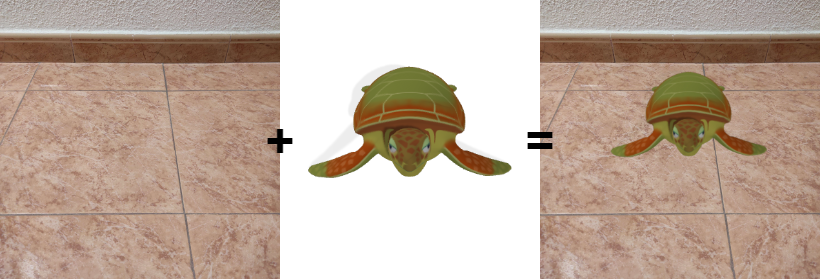
\includegraphics[width=0.8\textwidth]{img/sample_ra_schema.png}
        \caption{Ejemplo de superposición de imágenes en una \ra. La pose de la figura en 3D se calcula en relación con la imagen de la cámara para que su posición resulte fidedigna.}
        \label{fig:sample_ra_schema}
        \end{figure}

        Teniendo esto en cuenta, es importante que la renderización de la figura se realice con un fondo transparente o \textit{alfa}: cuando solicitemos al renderizador que nos genere una imagen, tendremos que indicarle el tamaño que tendrá dicha imagen para que concuerde con el tamaño de la pantalla. Este, generalmente, coincidirá con el tamaño de la imagen que capte la cámara, por lo que tendremos dos imágenes con el mismo tamaño solapándose en pantalla. Si queremos que la superposición tenga algún efecto visual, lo ideal es que el fondo de la imagen superior tenga un fondo transparente de forma que, si lo colocamos sobre cualquier otra imagen (como es el caso), se pueda observar sin problema la imagen inferior alrededor de la superior, como en el ejemplo de la figura \ref{fig:tortuga_marina}.
        
        \paragraph{}
        Parte de esta información se establece en el código \ref{lst:3.2}, a través de las opciones que se le indican al renderizador al ser inicializado en la línea 14. Antes de ser inicializado, se genera el objeto \textit{RENDEREROPTIONS} con elementos estáticos (fuera de la función) en la línea 2, donde se le indica que el fondo sea transparente a través de la propiedad de la línea 3. A mayores, dentro de la función se establecen otras propiedades que necesariamente se necesitan en tiempo de ejecución, como son en este caso los objetos \textit{canvas} y \textit{gl} (el contexto del \textit{canvas}), de los que ya tratamos previamente en la sección \ref{sec:sesion_webxr}. Esto se hace para que, al renderizar, se apliquen directamente los cambios sobre el \textit{canvas} que creamos para añadir los gráficos.

        \paragraph{}
        A continuación, se inicializa en la línea 17 la cámara virtual que utilizaremos durante la Sesión. A mayores de la propia inicialización, se le modifica el valor de una de sus propiedades en la línea siguiente: \textit{matrixAutoUpdate}. Esta propiedad heredada del objeto Object3D (objeto del que heredan también los objetos de Mallas anteriormente tratados), cuando se establece como verdadero, establece la posición, rotación y escala del elemento en cuestión en cuanto siente un cambio en estos, a ser posible en el fotograma en el que se realiza el cambio. Sin embargo, nosotros estableceremos el valor como false para poder indicar el fotograma exacto en el que queremos dicho cambio, evitando así que el sistema haga estos cambios en momentos inesperados.
        
        \paragraph{}
        Finalmente, en la línea 24, se inicializa un objeto muy importante que, aunque no forme parte de la librería \threejs, es necesario explicarla. El espacio de referencia, o Reference Space, es una definición de los sistemas de coordenadas que serán utilizados, en nuestro caso, dentro de la propia Sesión de \ra \cite{web:webxr_referencespace}. Lo que esto quiere decir es que, a través de los sensores de movimiento del dispositivo móvil, el sistema traducirá (o intentará traducir) en todo momento la información recibida en datos de movimiento y posición del mismo, y utilizará esto para calcular en todo momento dónde está el punto en el espacio que ha calculado como referencia, o dicho de otro modo, la coordenada $(0,0,0)$. Dicho de una manera resumida, el espacio de referencia es un sistema de coordenadas que tiene como punto 0 el lugar donde se inicia la Sesión, y el sistema mediante los sensores del dispositivo tratarán de calcular dónde está en todo momento el punto 0 y, a partir de este, tratarán de calcular las coordenadas del mismo dispositivo. Una vez sepa el dispositivo <<dónde está>>, será capaz de calcular también donde están otros objetos a los que se les ha dado también coordenadas en el espacio.

        \paragraph{}
        Será este espacio de referencia el que utilicemos para colocar objetos a nuestro alrededor y poder mantener la referencia de su ubicación y pose. Para ello, primero se define qué tipo de espacio de referencia se va a utilizar. La documentación de \webxr define varios tipos de espacios de referencia, pero recomienda concretamente \textit{local} para casos en los que el usuario no se vaya a alejar mucho del punto de origen y esté sentado (o cerca del suelo). En nuestro caso, no podemos saber si el usuario va a estar de pie o sentado, lo que podría suponer un debate entre usar \textit{local} o usar \textit{local-floor}, pero la misma documentación también nos indica que no existe una gran diferencia entre los dos tipos, al indicarnos que la diferencia sustancial entre ambos es que en el primero el punto 0 se genera cerca del punto donde estaba el dispositivo cuando se inició la Sesión y en el segundo se genera procurando acercar la coordenada \textit{y} cerca del suelo, lo que para este sistema no va a suponer una variación significativa. Por otro lado, la documentación sí establece las similitudes, al definir a ambos como los tipos de espacio de referencia en los que el usuario se mantendrá cerca del origen o se desplazarán a poca distancia del mismo, por lo que el sistema se optimizará para mantener con la mayor precisión posible el punto 0 y mantenerlo estable en relación a las variaciones de posición del mismo usuario.

        \paragraph{}
        Por último, y para terminar con los espacios de referencia, cabe mencionar que el espacio de referencia se solicita a través de una función del objeto que contiene nuestra Sesión. De esta manera, la librería facilita la comunicación del sistema con los detectores de posición y movimiento del móvil al devolver una interfaz que contiene toda la información necesaria. Esta llega a través de una promesa para los casos en que sea necesario recibir la interfaz de manera asíncrona. Sin embargo, en el momento en que se solicita, nuestro sistema está preparando el bucle de renderizado, el cual es un momento crítico donde muchos elementos tienen que estar preparados para que nada falle. Por lo tanto, se esperará a que esta promesa finalice y devuelva el espacio de referencia utilizando \textit{await}, de manera que el sistema no pase a la siguiente orden hasta que finalice la función \textit{requestReferenceSpace}. Una vez termine, podremos solicitar el primer fotograma a través de la función de la línea 28 explicada previamente en la sección \ref{sec:procesado_iterativo}.

        \paragraph{}
        Una vez solicitado el primer fotograma, se comenzará a ejecutar la función \textit{callback} para procesado de fotogramas en bucle, hasta que el usuario decida pararlo. En esta función, las acciones que realizaremos relacionadas con la librería \threejs estarán orientadas al posicionamiento de los modelos en 3D que mostremos usando \ra y a su renderizado. Como se hizo antes, se dejará comentado el código ya visto para evitar que quede demasiado extenso:

        \begin{lstlisting}[language=JavaScript, caption={Uso de la librería Three.js durante el bucle de renderizado.}, label={lst:3.3}]
#loopFunction = (time, frame) => {
    // ...
    
    // Solicitud de siguiente fotograma y enlazado de imagen de camara con modelo
    // ...
    
    // Calculo de posicion del usuario
    const pose = frame.getViewerPose(this.#referenceSpace);
    if (pose) {
        const view = pose.views[0];
        
        // Establecimiento de las proporciones de las imagenes renderizadas
        const viewport = this.#session.renderState.baseLayer.getViewport(view);
        this.#renderer.setSize(viewport.width, viewport.height);
        // ...
        
        // Posicion virtual del usuario para la vista
        this.#camera.matrix.fromArray(view.transform.matrix);
        this.#camera.projectionMatrix.fromArray(view.projectionMatrix);
        this.#camera.updateMatrixWorld(true);
        // ...

        // Posicion de la reticula
        this.#reticle.position.set(0.0, 0.0, 0.0); // stub
        this.#reticle.updateMatrixWorld(true); // stub
        // ...
        
        // Aplica las imagenes
        this.#renderer.render(this.#scene, this.#camera);
    }
};
\end{lstlisting}

        En el bucle, utilizaremos el objeto \textit{frame} descrito por primera vez en la sección \ref{sec:procesado_iterativo} para obtener datos del dispositivo que nos servirán para calcular cómo se debe renderizar la figura 3D. En primer lugar, debemos conseguir la \textit{pose} del móvil, que es la posición y orientación de este mismo. Para esto, es necesario utilizar el espacio de referencia que creamos en el código \ref{lst:3.2}, y se obtendrá mediante la función \textit{getViewerPose} de la clase \textit{XRFrame} (lo que es nuestro objeto \textit{frame}) utilizada en la línea 8. Esta función nos devolverá un objeto de la clase \textit{XRViewerPose} \cite{web:mozilla_xrviewerpose}, que representa la posición y orientación de la vista del espectador dependiendo del tipo de sesión que esté utilizando. En caso de que el usuario haya iniciado una sesión de \rv, el objeto generará dos posiciones distintas, una por cada ojo, para que por cada vista se pueda realizar la renderización correcta y la sensación de tridimensionalidad sea buena. En cambio, la sesión de \ra solo tiene un <<ojo>>, que es el objetivo de la cámara, por lo que la posición que devuelve tiene que representar la posición de este objetivo.

        \paragraph{}
        Una vez tenemos esto, procedemos a utilizar su información. En la línea 9 nos aseguramos de que la función \textit{getViewerPose} nos haya devuelto el objeto. Si es así, podremos obtener de él el objeto \textit{XRView} \cite{web:mozilla_xrview}, que contendrá la posición y orientación de nuestro objetivo, lo que nos permitirá calcular su <<punto de vista>>: qué puede ver, desde qué ángulo lo ve, a qué distancia lo ve, etc. Además, en la línea 13, solicitaremos a la sesión que nos dé la información sobre la proporción de imagen que debemos utilizar. La función usada (\textit{getViewport}), recibe la vista porque, en los casos de sesiones de \rv, cada vista devolverá información distinta: el objeto \textit{XRViewport} contiene el ancho y el alto de la imagen que se generará, así como la posición de esta (punto \textit{x} y punto \textit{y} en la pantalla). Esto es porque, en las sesiones de \ra en los dispositivos móviles, a diferencia de la tecnología 3D utilizada en cines, se separa la vista de cada ojo en cada mitad de la pantalla del móvil para utilizar gafas de tipo \textit{Google Cardboard}, que son lentes muy sencillas que aislan a cada ojo de la imagen que debe ver el otro y que, además, aumentan la imagen para que sea natural al ojo humano. Dado que este no será el caso, solo nos interesará el ancho y el alto de la imagen proporcionados por el \textit{viewport} para utilizarlo en el renderizador de \threejs, de manera que todas las imágenes que se generen tengan las mismas proporciones. Esto se lo explicitaremos en la línea 14 utilizando la función \textit{setSize} sobre el objeto \textit{renderer} que se inicializó en el código \ref{lst:3.2}.

\begin{figure}
\centering
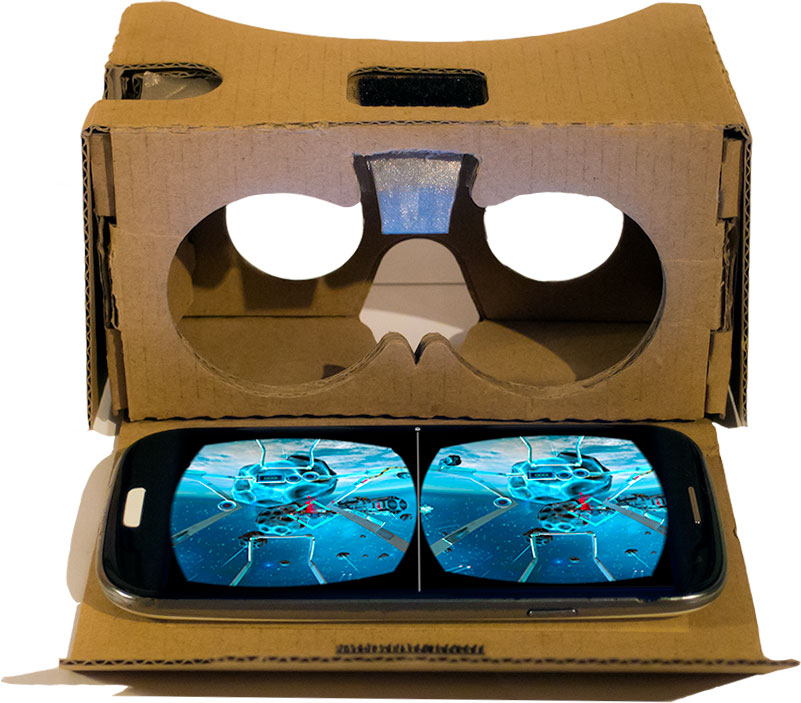
\includegraphics[width=0.5\textwidth]{img/google_cardboard.jpg}
\caption{Ejemplo de uso de las \textit{Google Cardboard} para visualizar contenido en \rv. Imagen extraída de A Principal's Reflections (Blogspot).}
\label{fig:google_cardboard}
\end{figure}

        \paragraph{}
        A continuación, se establecen las propiedades de la cámara virtual \cite{web:threejs_perspectivecamera}: mediante la función usada en la línea 18, se establece la posición del objetivo, así como su orientación; en la línea 19 se establecerán las coordenadas de proyección, que serán las que establezcan cuánto y cómo reducirán su tamaño las figuras en relación a la distancia a la que estén \cite{web:mozilla_xrview}; y en la línea 20 se fuerza a la cámara a actualizar estos cambios, de manera que los tengamos en cuando se genere la próxima renderización con el objeto \textit{renderer} al final de la función.

        \paragraph{}
        En último lugar, en la línea 24, se establece la posición de la figura \cite{web:threejs_object3d}. En este caso, como ejemplo, se establece la posición en $(0, 0, 0)$, de manera que, si se iniciara la sesión con esta configuración, la figura estaría estática en el aire, muy cercana al punto donde se encontraba el móvil cuando se inició la sesión. En la siguiente sección, se realizará la configuración para que la retícula se encuentre siempre en el suelo y funcione como <<puntero>> para saber dónde se ubicarán otras figuras. Una vez establecidos los datos de esta figura, también actualizaremos sus datos usando la función \textit{updateMatrixWorld}.

        \paragraph{}
        Para finalizar el procesado y juntar la parte \textit{real} con la \textit{virtual}, simplemente será necesario pedirle al \textit{renderer} que renderice las figuras \cite{web:threejs_webglrenderer} para que esta, de manera automática al contener la referencia al canvas y a su contexto desde su inicialización en el código \ref{lst:3.2}, las añada, finalizando así la formación del fotograma con nuestra figura añadida.

        \paragraph{}
        Ahora, hasta este punto, el comportamiento debería ser el siguiente: el usuario entraría en la página, pulsaría el botón de iniciar sesión de \ra y se mostraría la imagen obtenida por cámara. Cuando el sistema termine de cargar la retícula, esta se mostrará de manera fija en el espacio, muy cercano al punto donde el usuario inició la sesión. Con esto ya montado, es el momento de aumentar la funcionalidad, comenzando por el cálculo de superficies.

        \section{Cálculo de superficies, \textit{Hit Test Results}}
        \label{sec:calculo_de_superficies_hit_test_results}
        La siguiente característica a desarrollar es la capacidad del usuario para ubicar el avatar en el lugar que desee, estando siempre encima de una superficie, de manera que dé la sensación de estar esta reposando sobre el plano que hayamos seleccionado. Para ello se utilizará las herramientas proporcionadas por \webxr en conjunto con \threejs para poder encontrar superficies y apuntar hacia estas.

        \paragraph{}
        En este punto, será de gran importancia la retícula, la figura que se ha estado usando como ejemplo de modelo 3D para la carga y la inserción en este sistema de \ra. Esta figura se utilizará como puntero para que el usuario sepa en todo momento hacia dónde está apuntando, situándose esta en el punto de la superficie que se muestre exactamente en el centro de la pantalla. Para encontrar las coordenadas de dicho punto en la superficie, se utiliza \hittest.

\begin{figure}
\centering
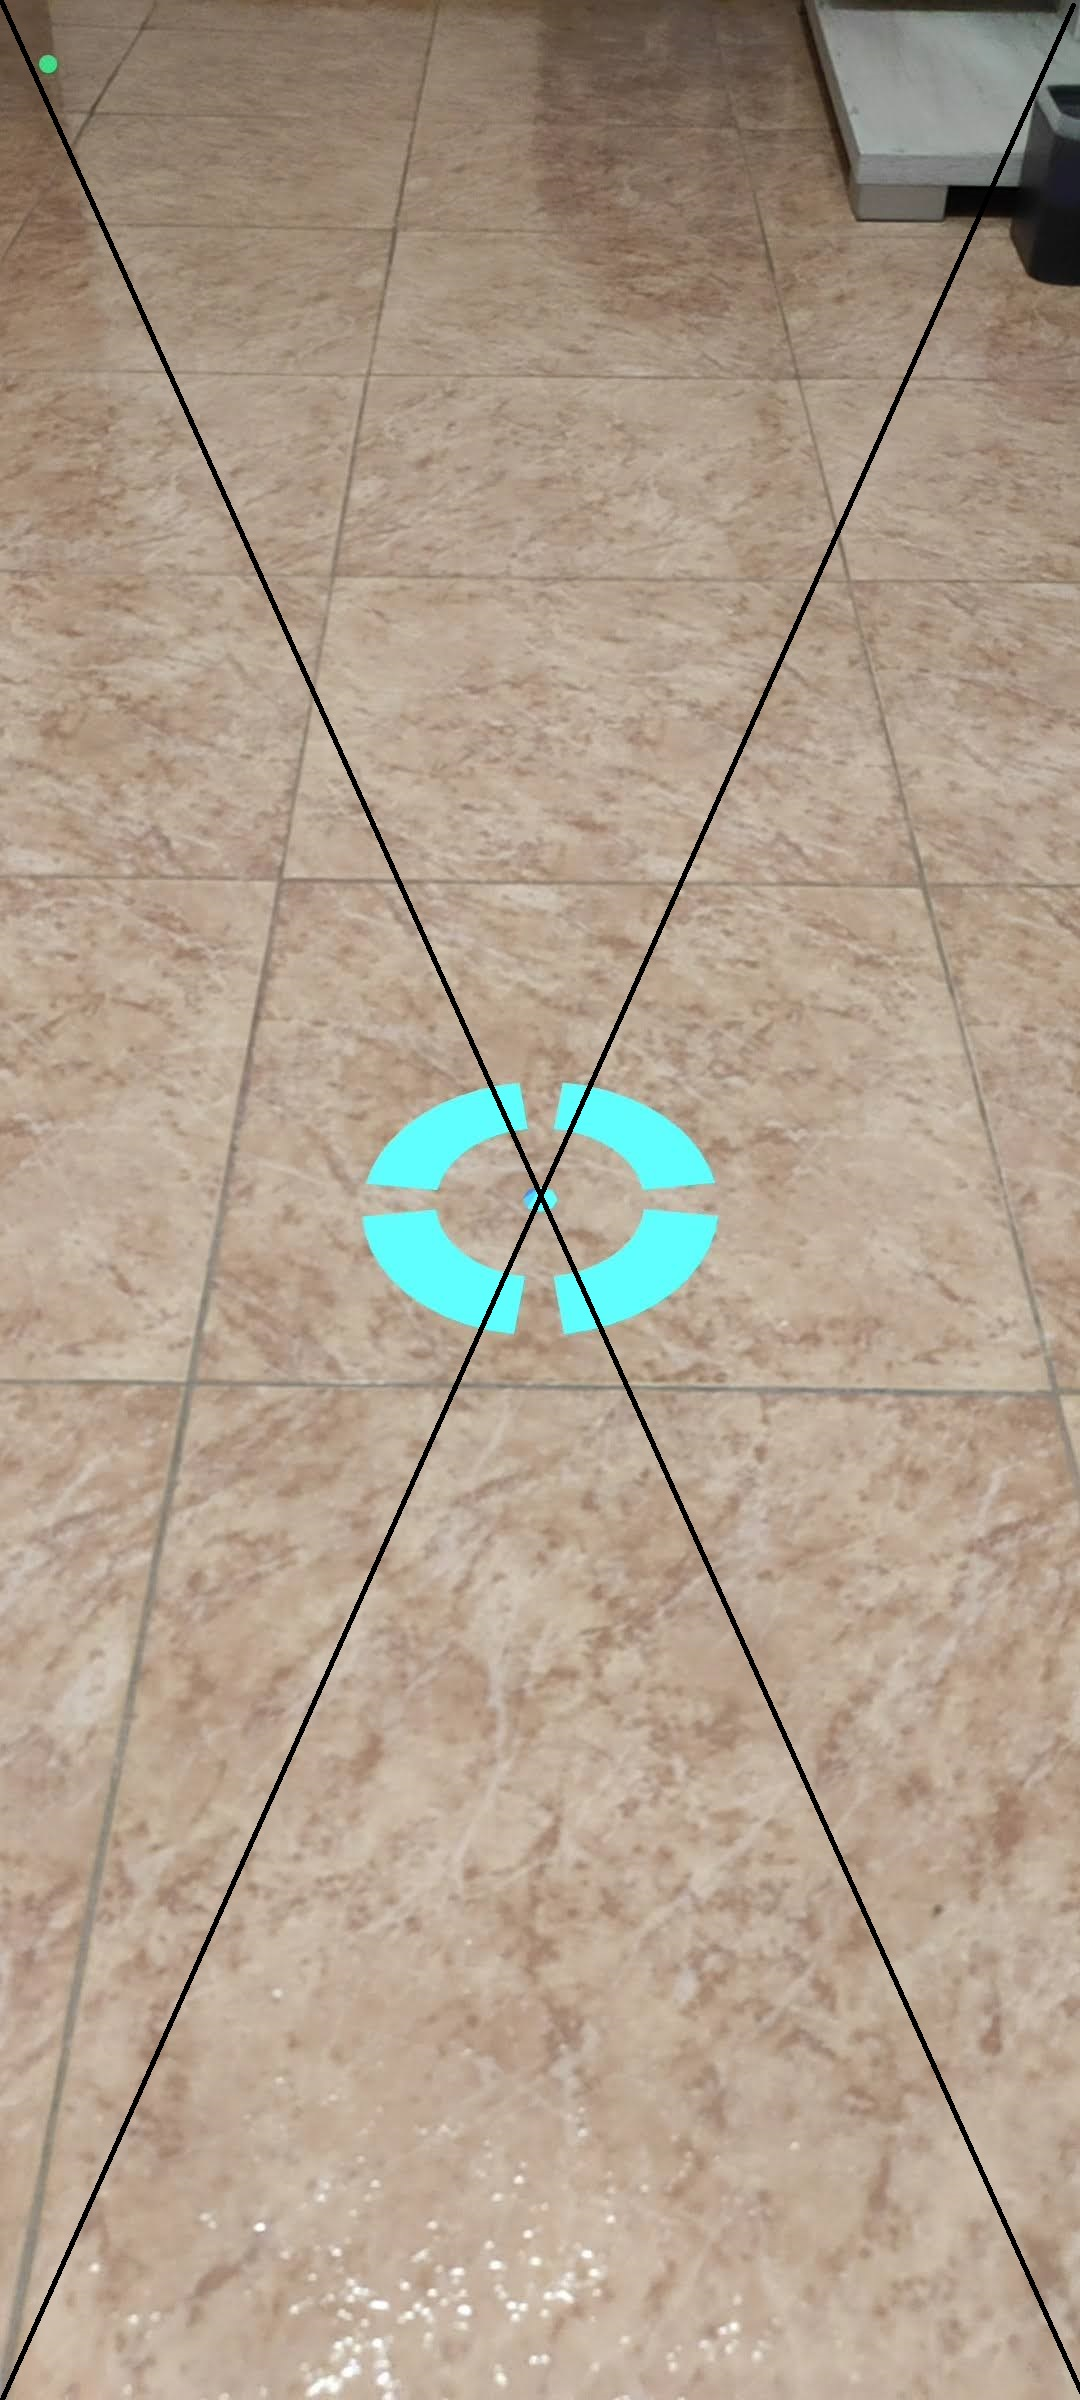
\includegraphics[width=0.25\textwidth]{img/hit-test-example.jpg}
\caption{\hittest devuelve la posición  de la superficie que se encuentre en el centro de la pantalla.}
\label{fig:hit-test-example}
\end{figure}

        \paragraph{}
        \hittest es una técnica que consiste en encontrar intersecciones entre superficies de objetos 3D y un rayo imaginario que, en el caso de esta aplicación, surgirá desde el dispositivo móvil. En el caso de los sistemas que utilizan \rv, el cálculo se realiza teniendo en cuenta que se conocen previamente los objetos que generarán las intersecciones, pero a la hora de utilizar \ra, este proceso resulta algo más complejo, al ser necesario encontrar la forma que tienen los objetos de nuestro alrededor para poder realizar los cálculos. Afortunadamente, la interfaz \webxr cuenta con las herramientas adecuadas para hacer estos cálculos internamente, de forma que los desarrolladores solo tengan que ocuparse de tratar la información que devuelvan los resultados del \hittest.

        \paragraph{}
        Es importante tener en cuenta que los resultados del \hittest pueden depender de la calidad de los sensores y cámaras del dispositivo. Además, la experiencia puede variar en diferentes entornos y condiciones de iluminación, por lo que las coordenadas obtenidas a través de esta técnica puede variar ampliamente dependiendo de cada casuística.

        \paragraph{}
        Conociendo ya esto, vamos a su aplicación en el sistema desarrollado. Para comenzar, es necesario indicar a la Sesión, cuando esta esté siendo creada, que se va a utilizar las opciones de \hittest y que se requerirá cargar la configuración necesaria para su utilización. Para ello, se utiliza el objeto \textit{SESSIONOPTIONS} que contiene información sobre cómo deberá ser la Sesión creada. En este caso, como ya se mostró anteriormente en el código \ref{lst:2.4}, la opción a indicar es \textit{requiredFeature}, y dentro de esta indicaremos mediante String que queremos que la sesión use \textit{'hit-test'}.

        \paragraph{}
        Después de esto, dentro de la función \textit{startLoop}, tendremos que obtener un espacio de referencia que pueda utilizar el sistema para poder calcular las intersecciones. En este caso, se utilizará un espacio de referencia de tipo \textit{viewer} \cite{web:webxr_referencespace}, ya que es un espacio de referencia centrado en ubicar el suelo. Con esto, podemos solicitar a la sesión que nos ofrezca un \hittestsource. El \hittestsource nos permitirá, cuando nos encontremos en el bucle, encontrar en nuestro espacio de referencia las coordenadas del punto de la superficie al que apuntamos con la cámara, tal y como se hace en la imagen \ref{fig:hit-test-example} \cite{web:mozilla_xrhittestsource}. En el código \ref{lst:3.4}, en la línea 18, justo después de la solicitud del espacio de referencia que va a utilizar y junto al otro espacio de referencia utilizado por la aplilcación, se muestra la solicitud de dicho objeto, que se realiza a través de una llamada asíncrona, razón por la cual se utiliza el comando \textit{await}.

\paragraph{}
\begin{lstlisting}[language=JavaScript, caption={Solicitud de Hit Test Source a la Sesión y creación de evento.}, label={lst:3.4}]
async startLoop() {

    // ...

    // Session
    this.#session = await navigator.xr.requestSession("immersive-ar", this.#SESSIONOPTIONS);
    this.#session.updateRenderState({
        baseLayer: new XRWebGLLayer(this.#session, this.#gl)
    });

    // Reference space
    this.#referenceSpace = await this.#session.requestReferenceSpace('local');

    // Viewer space
    this.#viewerSpace = await this.#session.requestReferenceSpace('viewer');

    // Hit test source
    this.#hitTestSource = await this.#session.requestHitTestSource({ space: this.#viewerSpace });

    //...

    this.#session.addEventListener("select", this.#onTouchEvent);

    // ...
    
}
\end{lstlisting}

        Antes de terminar con la función \textit{startLoop}, prepararemos un evento que servirá para aplicar la funcionalidad de la aplicación que funciona gracias a \hittest. Como vemos en la línea 22 del código \ref{lst:3.4}, mediante la función \textit{addEventListener} de la Sesión, solicitaremos que se fije un evento de tipo \textit{<<select>>}, lo que significa que cada vez que se pulse la pantalla con la sesión iniciada, se lanzará la función de tipo \textit{callback} especificada en el segundo parámetro llamada \textit{onTouchEvent}. Concretamente, como respuesta a este evento, el sistema lanzará el siguiente código:

\begin{lstlisting}[language=JavaScript, caption={Respuesta al evento de tipo <<select>>.}, label={lst:3.5}]
#onTouchEvent = (event) => {
    if (this.#model) {
        this.#scene.remove(this.#model)
        this.#model.position.copy(this.#reticle.position);
        this.#scene.add(this.#model);
        
        // ...
    }
};
\end{lstlisting}

        \paragraph{}
        En el código \ref{lst:3.5}, lanzado cada vez que el usuario toca la pantalla, eliminaremos del Escenario la retícula mediante la línea 3. A efectos prácticos, esto significa que la retícula desaparecerá por completo de nuestra \ra, siendo imposible volver a encontrarla. Sin embargo, esto solo ocurrirá si se cumple la condición de la línea 2, que comprueba si se ha cargado la variable \textit{model}. Esta variable contiene otra figura 3D, que en este caso es el modelo de nuestro asistente virtual. Esta se comenzará a cargar a la vez que la retícula, pero debido a que este modelo 3D pesa mucho más y su carga se realiza de manera asíncrona, es necesario comprobar que se ha terminado de cargar antes de utilizarlo. Por esta razón, se lanza la comprobación de la línea 2: debido a que \js interpreta las variables vacías como \textit{false} y cualquier contenido (no booleano) como \textit{true} \cite{web:mozilla_booleanevaluation}, al leer esa condición, el sistema solo pasará por el condicional si la variable ha sido cargada. Esta carga asíncrona se realiza en la función \textit{checkSessionSupported()} y se explicará con más detalle en la sección \ref{sec:calculo_de_superficies_hit_test_results}.
        
        \paragraph{}
        Una vez se evalúa afirmativamente la condición de la línea 2, como ya se ha dicho, se quitará la retícula del Escenario. Pero para continuar con la funcionalidad de la aplicación, se procede también con las otras dos líneas: nuestra aplicación debe mostrar el modelo cargado en la variable \textit{model} en el mismo punto exacto en el que se encontraba la retícula en el momento en que el usuario pulsó sobre la pantalla, por lo que el asistente virtual deberá tener exactamente la misma que la retícula con respecto a la posición. Para eso, se usa la función de la línea 4, que se encarga de copiar completamente dicha información. Por último, como queremos que aparezca el asistente virtual en nuestra pantalla, utilizaremos la función de la línea 5 para que esta sea añadida a la Escena y, por tanto, el sistema se encargue de renderizarlo en pantalla. Esta es la manera en que intercambiaremos un modelo por otro.
        
        %% TODO explicar la parte del hit test del bucle
        \paragraph{}
        Una vez obtenido todo lo necesario para iniciar nuestro \hittestsource, comenzaremos con la implementación en el bucle de la función \textit{loopFunction}. En el código \ref{lst:3.3}, se sustituyó contenido del script original por las líneas 24 y 25 para poder explicar mejor su funcionamiento, pero ahora que se ha explicado lo necesario para llegar a esto, mostraremos en el código \ref{lst:3.6} el contenido que originalmente va en esas líneas:

\begin{lstlisting}[language=JavaScript, caption={Obtención de valores captados a través del Hit Test Source.}, label={lst:3.6}]
// ...
// Calculo de superficies
const hitTestResults = frame.getHitTestResults(this.#hitTestSource);
if (hitTestResults.length > 0 && this.#reticle) {

    const hitPose = hitTestResults[0].getPose(this.#referenceSpace);
    
    // muestra la reticula solo si esta cargado el modelo y no esta hablando
    if (this.#model && !this.#clipAction.isRunning())
        this.#reticle.visible = true;
    else
        this.#reticle.visible = false;
    
    this.#reticle.position.set(hitPose.transform.position.x, hitPose.transform.position.y, hitPose.transform.position.z)
    this.#reticle.updateMatrixWorld(true);
    
}
// ...
\end{lstlisting}

        \paragraph{}
        En primer lugar, en la línea 3, se solicita al objeto \textit{frame} que devuelva el resultado de los cálculos usando el \hittestsource mediante la función \textit{getHitTestResults}. Los resultados serán unas coordenadas que indicarán la posición aproximada del punto de la superficie a la que se esté apuntando con la cámara del dispositivo. Una vez realizada esta función, se comprueba si ha devuelto algún valor mediante la condición de la línea 4. Esto se hace porque es posible que comience el bucle pero el sistema todavía no haya captado correctamente el sistema de referencia y, por tanto, todavía no pueda obtener resultados de superficies. Además, al igual que se hizo en el código \ref{lst:3.5}, también se comprueba que se haya terminado de cargar la retícula para poder mostrarla en pantalla. Si ambas condiciones se dan, se pasa a dar a la retícula sus coordenadas: en la línea 6 se obtiene, del objeto <<resultados>>, las coordenadas que queremos asignar a cualquier modelo tridimensional a través de la función \textit{getPose}. En las líneas 9 y 11 se establecen las condiciones que indicarán si la retícula es o no visible durante la sesión del usuario y, finalmente, a través de la función de la línea 14, se establece la posición de la retícula cogiendo las coordenadas recibidas anteriormente del objeto <<resultados>>. Esta acción se realizará en cada iteración para asegurar que la retícula aparece siempre en la posición hacia la que está apuntando el usuario.

        \paragraph{}
        Con todo esto, el usuario ya podría ubicar objetos en superficies del mundo real a través de la \ra. El siguiente punto será animar dichos objetos.

        
        \section{Animación de modelos}
        \label{sec:animacion_de_modelos}
        La creación de animaciones de cada modelo, en el caso de este \tfg, se hace durante el propio diseño del modelo, punto que será tratado en el capítulo \ref{chap:4}. Sin embargo, es importante conocer esto, ya que algunos formatos de modelos en 3D como \glb o \gltf permiten almacenar dichas animaciones de manera que, al cargar los modelos, se puede utilizar también estas animaciones. En nuestra situación, son los modelos humanos los que contienen animaciones, debido a que la retícula no necesita ninguna.

        \paragraph{}
        Para comenzar con la animación de modelos, es necesario volver otra vez a la carga de los modelos, en la función \textit{checkSessionSupported}. En este caso, trataremos concretamente la animación de los modelos humanos que, como se ve en el código \ref{lst:3.7}, es algo distinto a la carga de la retícula.

\newpage
\begin{lstlisting}[language=JavaScript, caption={Carga de modelo humano.}, label={lst:3.7}, float=ht]
#MODELLINKARRAY = ["resources/model/stormy-male.glb", "resources/model/stormie-female.glb"];
#ANIMATIONLOOP = false;
// ...

#checkSessionSupported = (isSupported) => {
    if (isSupported) {
        // Model
        this.#modelSelected = Math.floor(Math.random() * this.#MODELLINKARRAY.length);
        this.#modelLink = this.#MODELLINKARRAY[parseInt(this.#modelSelected)];

        // Scene y Loader
        this.#scene = new THREE.Scene();
        this.#loader = new THREE.GLTFLoader();
        this.#clock = new THREE.Clock(this.#CLOCKAUTOSTART);

// ...

        // Modelo
        this.#loader.load(this.#modelLink, function(gltf) {
            // Figura
            this.#model = gltf.scene;
            this.#model.name = this.#MODELNAME;
            this.#model.scale.set(this.#MODELSCALE.x, this.#MODELSCALE.y, this.#MODELSCALE.z);

            // Animacion
            this.#mixer = new THREE.AnimationMixer(this.#model);

            let jsonAnimations = gltf.animations;
            this.#clipAction = this.#mixer.clipAction(jsonAnimations[this.#MODELANIMATIONNUMBER]);
            if (!this.#ANIMATIONLOOP) {
                this.#clipAction.setLoop(THREE.LoopOnce); // playing the clip once
                this.#clipAction.clampWhenFinished = true;
                this.#clipAction.enable = true;
            }
        }.bind(this));
    } 
// ...
};
\end{lstlisting}

        Una peculiaridad de la carga de los modelos humanos es que, de los dos modelos que tenemos, se cargará uno de ellos de manera aleatoria, sin aplicar ningún tipo de decisión más allá del uso de un número calculado aleatoriamente. Esto se realiza de la siguiente manera: en la línea 1, se almacena la constante con las ubicaciones de los dos modelos en un \textit{array} de cadenas de texto. Más tarde, justo antes de realizar las cargas, se decide qué modelo se va a utilizar, usando para ello en la línea 7 la librería \textit{Math} para calcular un número entero de manera aleatoria y que permita seleccionar, en la línea 8, la posición del \textit{array} (en este caso, la posición será 0 o 1).

        \paragraph{}
        Una vez calculado qué modelo se va a utilizar, se pasa a la función \textit{load} ya comentada en la sección \ref{sec:modelo_en_3d_y_three_js} donde, a través de una función \textit{callback}, se obtiene un objeto con el que se podrá manipular el modelo 3D. Ya obtenido este, se comienza a configurar: se almacena la Escena devuelta, se le asigna un nombre reconocible a su atributo \textit{name} y se le da el tamaño deseado en el atributo \textit{scale}.

        \paragraph{}
        Una vez tenemos el objeto del modelo, comenzamos con el trabajo de tratamiento de la animación. Para ello, utilizamos un objeto de la librería \threejs, \textit{AnimationMixer} \cite{web:threejs_animationmixer}, que contiene utilidades básicas de control de la animación, como la velocidad de reproducción de esta misma o, la más importante, la capacidad de buscar el momento exacto de la animación que debe mostrarse en relación al tiempo. De este objeto obtendremos también el objeto \textit{AnimationAction} \cite{web:threejs_animationaction} almacenado en la variable \textit{clipAction} en la línea 29, que permite un control de la animación más parecido a los controles globales de reproducción de vídeo: pausar, reanudar, establecer un bucle, establecer la duración de la animación, etc. Para poder utilizar este último, tendremos que pasarle la animación que se va a usar. Una vez obtenido, podremos configurarlo como se hace a partir de la línea 31, donde en este caso se establece que la animación no se ejecute continuamente en bucle, se indica que la animación se desactive al terminar y, finalmente, se activa dicha animación.

        \paragraph{}
        Por último, antes de lanzar la función \textit{load} de la línea 19, se prepara un objeto llamado \textit{Clock} \cite{web:threejs_clock}. Este objeto sirve para contar los segundos que lleva la animación reproduciéndose y, en el momento de renderizar la figura, \textit{AnimationMixer} la actualice para que se encuentre en la posición en la que debe estar en el tiempo indicado por el reloj. Este objeto es necesario debido a que, tal y como se comentó anteriormente en la sección \ref{sec:procesado_iterativo}, cada fotograma se lanza únicamente cuando el sistema está preparado para lanzarlo en lugar de lanzarse todos los fotogramas posibles uno tras otro. Por lo tanto, debe haber un control que tenga en cuenta los segundos de ejecución que se llevan durante cada iteración y que, con esto, sepa qué instante exacto de la animación debe renderizarse.

        \paragraph{}
        Una vez están estos objetos preparados, se puede comenzar a utilizar en el propio trabajo de renderizado. El primer lugar en el que se utiliza es en \textit{onTouchEvent}:

\paragraph{}
\begin{lstlisting}[language=JavaScript, caption={Evento onTouchEvent junto con las acciones relacionadas con la animación.}, label={lst:3.8}]
#onTouchEvent = (event) => {
    if (this.#model) {
        this.#scene.remove(this.#model);
        this.#model.position.copy(this.#reticle.position);
        this.#scene.add(this.#model);
// ...
        if (!this.#clipAction.isRunning()) {
            this.#clipAction.setDuration(this.#audioElement.duration);
            this.#clipAction.reset();
            this.#clipAction.play();
        }
    }
};
\end{lstlisting}

        Aquí, cuando el usuario pulsa sobre la pantalla, después de ejecutarse las acciones comentadas anteriormente en el código \ref{lst:3.5}, se comprueba primero que el modelo esté ejecutando su animación (línea 10) y, de no ser así, comienza con esta (línea 13). Antes de reproducirse, se realizan dos acciones: la primera, en la línea 11, establece la duración de la animación en relación con el audio que sonará a su vez. Esto se hace para, por un lado, fijar la velocidad a la que se ejecutará la animación (y asegurarse de que siempre va a ser la misma) y, por otro lado, para que cuadre con el mismo audio, ya que la animación se ha diseñado en relación a esta, como se comentará más adelante. La segunda acción, en la línea 12, se asegura de que, en caso de que la animación se haya detenido porque ya se había ejecutado y terminado por completo, la próxima vez que se inicie la animación se ejecute desde el punto de inicio en lugar de iniciarse desde el final o desde algún punto intermedio. De esta manera, el evento se ocuparía de iniciar la animación tanto si el usuario acaba de entrar en la \ra como si ha terminado la animación y quiere volver a reproducirla.
        
        \paragraph{}
        Por último, durante el bucle de renderizado, para actualizar la posición de la animación a la conveniente en el momento de ser renderizado, sería tan sencillo como ejecutar el siguiente fragmento de código al inicio del método:

\paragraph{}
\begin{lstlisting}[language=JavaScript, caption={Actualización de la posición del modelo 3D antes de renderizar.}, label={lst:3.9}]
#loopFunction = (time, frame) => {

    let delta = this.#ANIMATIONSPEED * this.#clock.getDelta();
    if (this.#mixer)
        this.#mixer.update(delta);

// ...
};
\end{lstlisting}

        La función de la línea 5 se asegura, sin necesidad de ejecutar más acciones, de actualizar la posición del modelo. Para poder ser ejecutado, se extrae en la línea 3 el valor \textit{delta} del objeto \textit{Clock}, que es el tiempo en segundos que ha pasado desde que se inició el reloj. Además, en la línea 4 se comprueba que este código se ejecute únicamente si de manera previa se ha generado el objeto \textit{mixer} durante las acciones asíncronas en la preparación del bucle, como se vio en el fragmento de código \ref{lst:3.7}.
        
        \paragraph{}
        Con todo esto, ya dispondríamos de una aplicación de \ra que, a partir de las acciones del usuario, será capaz de posicionar modelos 3D con movimiento en superficies reales. Por último, quedaría añadir la última capa de verosimilitud mediante el sonido espacial.

        \section{Sonido espacial}
        \label{sec:sonido_espacial}
        Para aplicar el sonido espacial al sistema, como se mencionó en la sección \ref{sec:tecnologias_utilizadas}, se ha utilizado la librería \resonanceaudio \cite{web:resonance_audio}. Esta librería está especializada en la simulación de sonidos espaciales, de manera que un usuario con auriculares podría reconocer de dónde provienen las voces que escuchará a través de la aplicación. Otra funcionalidad que, además, se percibe sin necesidad de auriculares, es la <<pérdida de volumen>> en relación con la distancia al origen del sonido, con lo que seremos capaces de escuchar mejor a nuestro modelo si este está ubicado en nuestros alrededores, mientras que si se ubica a una gran distancia no seremos capaces apenas de escucharlo.

        \paragraph{}
        El uso de \resonanceaudio es bastante similar al uso de la librería \threejs en cuanto al uso de modelos y animaciones, debido a que ambos requieren ubicar un elemento en el espacio y, además, reproducirlo. En el caso del audio, el proceso de carga de archivos es mucho más sencillo.

\paragraph{}
\begin{lstlisting}[language=JavaScript, caption={Preparación del sonido espacial.}, label={lst:3.10}]
async startLoop() {

    // ...

    this.#audioContext = new AudioContext();

    this.#resonanceAudioScene = new ResonanceAudio(this.#audioContext);
    this.#resonanceAudioScene.output.connect(this.#audioContext.destination);
    this.#resonanceAudioScene.setRoomProperties(this.#ROOMDIMENSIONS, this.#ROOMMATERIALS);

    this.#audioElement = document.createElement('audio');
    this.#audioElement.src = this.#audioLink;
    this.#audioElement.loop = this.#AUDIOLOOP;

    this.#audioElementSource = this.#audioContext.createMediaElementSource(this.#audioElement);

    this.#audioSource = this.#resonanceAudioScene.createSource();
    this.#audioElementSource.connect(this.#audioSource.input);
    this.#audioSource.setPosition(0.0, 0.0, 0.0);

    // ...

    this.#session.requestAnimationFrame(this.#loopFunction);
}
\end{lstlisting}

        El proceso de carga y configuración del audio comienza en la función \textit{startLoop}, donde se van preparando los objetos de la librería y especificando las opciones que se van a utilizar. Para empezar, se requiere del objeto \textit{AudioContext} \cite{web:mozilla_audiocontext}, que forma parte de la funcionalidad básica de \js y permite cargar y reproducir elementos de audio. Este será inicializado en la línea 5 del código \ref{lst:3.10} para después poder inicializar en la línea 7 el propio objeto \textit{ResonanceAudio} \cite{web:resonance_audio_resonanceaudio} incluyendo al primero como argumento del constructor. Mediante el uso de este último, la aplicación será capaz de generar el efecto de distancia y movimiento del sonido espacial. Para asignarle una salida de audio, utilizaremos la función de la línea 8.

        \paragraph{}
        En la línea 9, se establecen las propiedades de la habitación: largo, ancho, altura del techo y materiales de cada una de las superficies \cite{web:resonance_audio_utils} (suponiendo que la habitación está formada por cuatro paredes paralelas, suelo y techo y omitiendo formas que no sean hexaédricas). En este caso, dado que no queremos simular el efecto de eco, se establece como dimensiones 0x0x0, que es la forma de decirle al sistema que la habitación no tiene una forma definida; y como materiales de paredes y techo se asigna el valor <<\textit{transparent}>>, lo que significa que no hay un material solido en dichas estructuras, mientras que para el suelo se establece <<\textit{marble}>>.

        \paragraph{}
        A continuación, en la línea 11, se crea un \textit{HTMLAudioElement} \cite{web:mozilla_htmlaudioelement} a través de la función \textit{createElement} del propio documento. Este elemento es una interfaz que permite insertar un audio en un documento HTML y que, a su vez, ofrece funciones de manipulación del mismo. Sobre este, estableceremos dos propiedades: la primera, \textit{src} (línea 12), servirá para ubicar el origen del archivo de audio que se reproducirá en la aplicación; la segunda, \textit{loop} (línea 13), indicará a la aplicación si, al terminar el audio, debe volver a reproducirse desde el principio automáticamente.

        \paragraph{}
        Finalmente, mediante el código de las líneas 15 y 17, terminamos de <<conectar>> el \textit{HTMLAudioElement} con el objeto de \resonanceaudio para que el primero sea el origen del sonido del segundo, y mediante la función de la línea 19, establecemos una posición provisional para el origen del sonido. De esta manera, tenemos preparada la configuración del sonido espacial, con lo que se puede comenzar a desarrollar la funcionalidad aplicada a esta aplicación.
        
        \paragraph{}
        En primer lugar, se definirá lo que ocurre en los casos en los que emisor y receptor del sonido se muevan. Esto se puede ver en el código \ref{lst:3.11}, donde la funcionalidad se divide en dos partes: en la primera, representada por las filas 12, 13 y 14, se calcula la posición del usuario (que se extrae de \textit{view.transform.matrix}) y se inserta en el objeto \textit{THREE.Matrix4} \cite{web:threejs_matrix4}, objeto que almacena una matriz de 4x4 y que representa la posición, orientación y rotación de una figura. Esta posición del usuario nos servirá para establecer la posición del receptor utilizando la función \textit{setListenerFromMatrix}, de manera que \resonanceaudio sepa desde dónde se está escuchando el audio reproducido. En la segunda parte, representada por la fila 17, se establece el origen del sonido utilizando la posición del modelo.
        
        \paragraph{}
        A pesar de que en el bucle se estén estableciendo coordenadas, hay que tener en cuenta que todo esto no afecta en la reproducción o pausa de los sonidos cargados. Por lo tanto, durante varias iteraciones de este, \resonanceaudio tendrá definidas estas coordenadas a modo de <<preparación>> para cuando comience la reproducción.

\paragraph{}
\begin{lstlisting}[language=JavaScript, caption={Control del sonido espacial en el bucle.}, label={lst:3.11}]
#loopFunction = (time, frame) => {

// ...

    const pose = frame.getViewerPose(this.#referenceSpace);
    if (pose) {
        const view = pose.views[0];

        // ...

        let userPosition = new THREE.Matrix4();
        userPosition.elements = view.transform.matrix;
        this.#resonanceAudioScene.setListenerFromMatrix(userPosition);

        // ...

        this.#audioSource.setFromMatrix(this.#model.matrix);
        this.#renderer.render(this.#scene, this.#camera)
    }
};
\end{lstlisting}

        La parte del código donde sí se comienza con la reproducción del sonido es, al igual que con la animación, en el evento \textit{onTouchEvent}. Estas dos acciones se hacen a la vez para que el audio y la animación estén en todo momento sincronizados.

\paragraph{}
\begin{lstlisting}[language=JavaScript, caption={Control del sonido espacial en el evento onTouchEvent.}, label={lst:3.12}]
#onTouchEvent = (event) => {
    if (this.#model) {
// Aqui iria parte del control de la animacion de modelo
    
        this.#audioElement.play();

// Aqui iria otra parte del control de la animacion de modelo
    }
};
\end{lstlisting}

        En este caso, solo habría una línea que comentar del código \ref{lst:3.12}, que es la línea 5, donde se lanza la función \textit{play} para reproducir el audio. Cabe decir que esta función no hace nada si el audio ya se está reproduciendo, por lo que, al igual que el resto del evento, está planteado para lanzar el audio solo si este ya ha terminado o todavía no se ha reproducido.

        \paragraph{}
        Por último, en el caso de que el usuario cierre la sesión de \ra, necesitaríamos indicar al sistema que debe finalizar también el audio, en caso de que este siga reproduciéndose. Para esto utilizaremos el evento \textit{onSessionEnd}, asociado a la sesión de \ra a la par que el evento \textit{onTouchEvent}. Tal y como vemos en el código \ref{lst:3.13}, las dos acciones que se realizan al cerrar la sesión serían, primero, pausar la reproducción y, segundo, establecer el tiempo en cero para que, si el usuario vuelve a iniciar la sesión, la reproducción siga por el mismo sitio.

        \paragraph{}
\begin{lstlisting}[language=JavaScript, caption={Control del sonido en el cierre de la sesión de Realidad Aumentada.}, label={lst:3.13}]
	#onSessionEnd = (event) => {
		/* the session has shut down */
		this.#audioElement.pause();
		this.#audioElement.currentTime = 0;
	};
\end{lstlisting}

        Con esto, ya podríamos simular el sonido espacial, con lo que tendríamos cubierta la última capa de \ra que queremos desarrollar.

        \section{Funcionamiento final de la Realidad Aumentada}
        \label{sec:funcionamiento_final_de_la_realidad_aumentada}
        El caso de uso principal del usuario será, generalmente, el siguiente:

\begin{figure}[H]
\centering

\includegraphics[width=0.25\textwidth]{1_landing_page.jpg}
\caption{El usuario accede a la landing page.}
\label{fig:1_landing_page}
\end{figure}

        \paragraph{}
        Nada más entrar en la aplicación, como se explicó anteriormente, el usuario podrá ver la \textit{landing page}, una página estática sencilla donde aparecerá un botón que servirá para cargar los modelos necesarios y lanzar la sesión de \ra (figura \ref{fig:1_landing_page}). 

\begin{figure}[H]
\centering
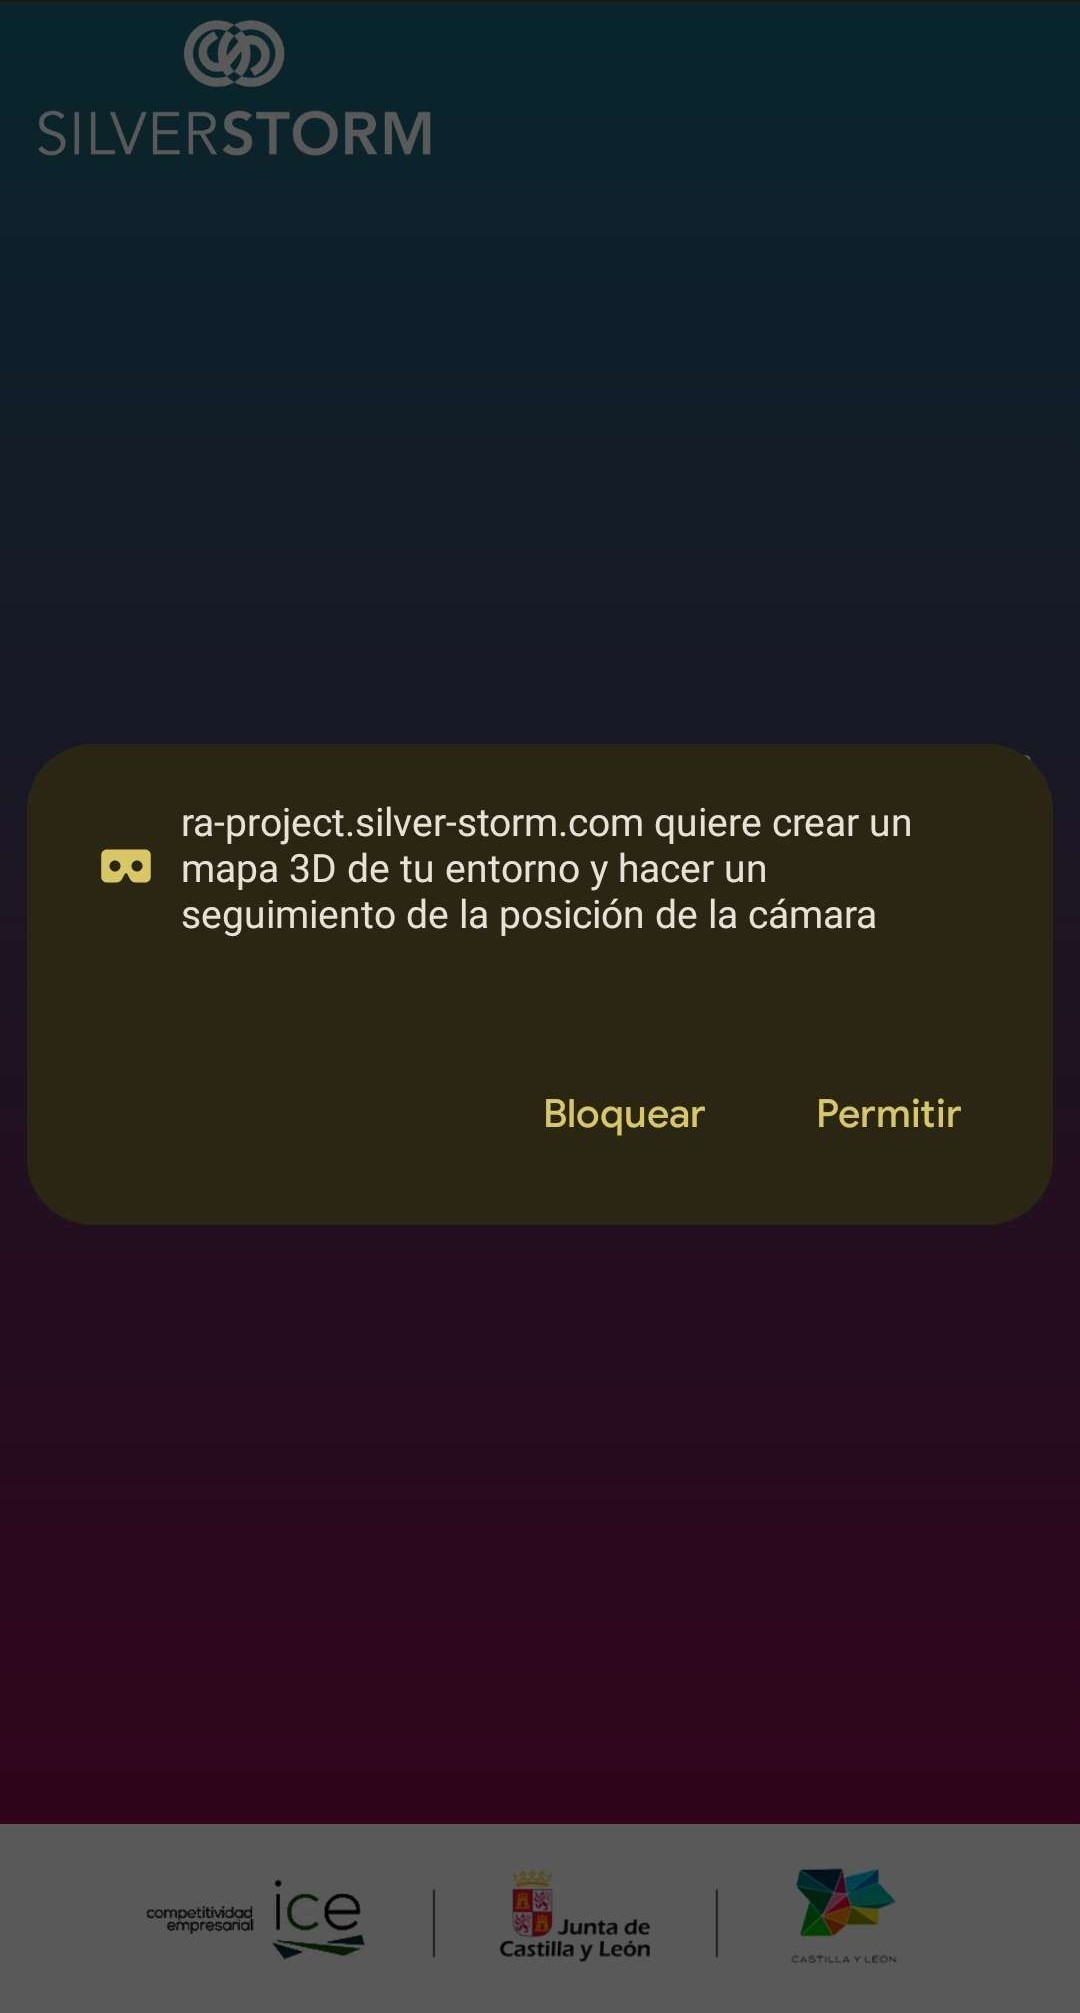
\includegraphics[width=0.25\textwidth]{2_permissions.jpg}
\caption{Se solicitan permisos al usuario.}
\label{fig:2_permissions}
\end{figure}

        \paragraph{}
        Al pulsar sobre el botón, el navegador avisará al usuario de que se pretenden utilizar funciones asociadas a la \ra (figura \ref{fig:2_permissions}). En concreto, el mensaje avisa al usuario sobre la posibilidad de crear mapas 3D del entorno y el seguimiento de la posición de la cámara. Si el usuario ha dado estos permisos previamente, el sistema no lo volverá a preguntar.

\begin{figure}[H]
\centering
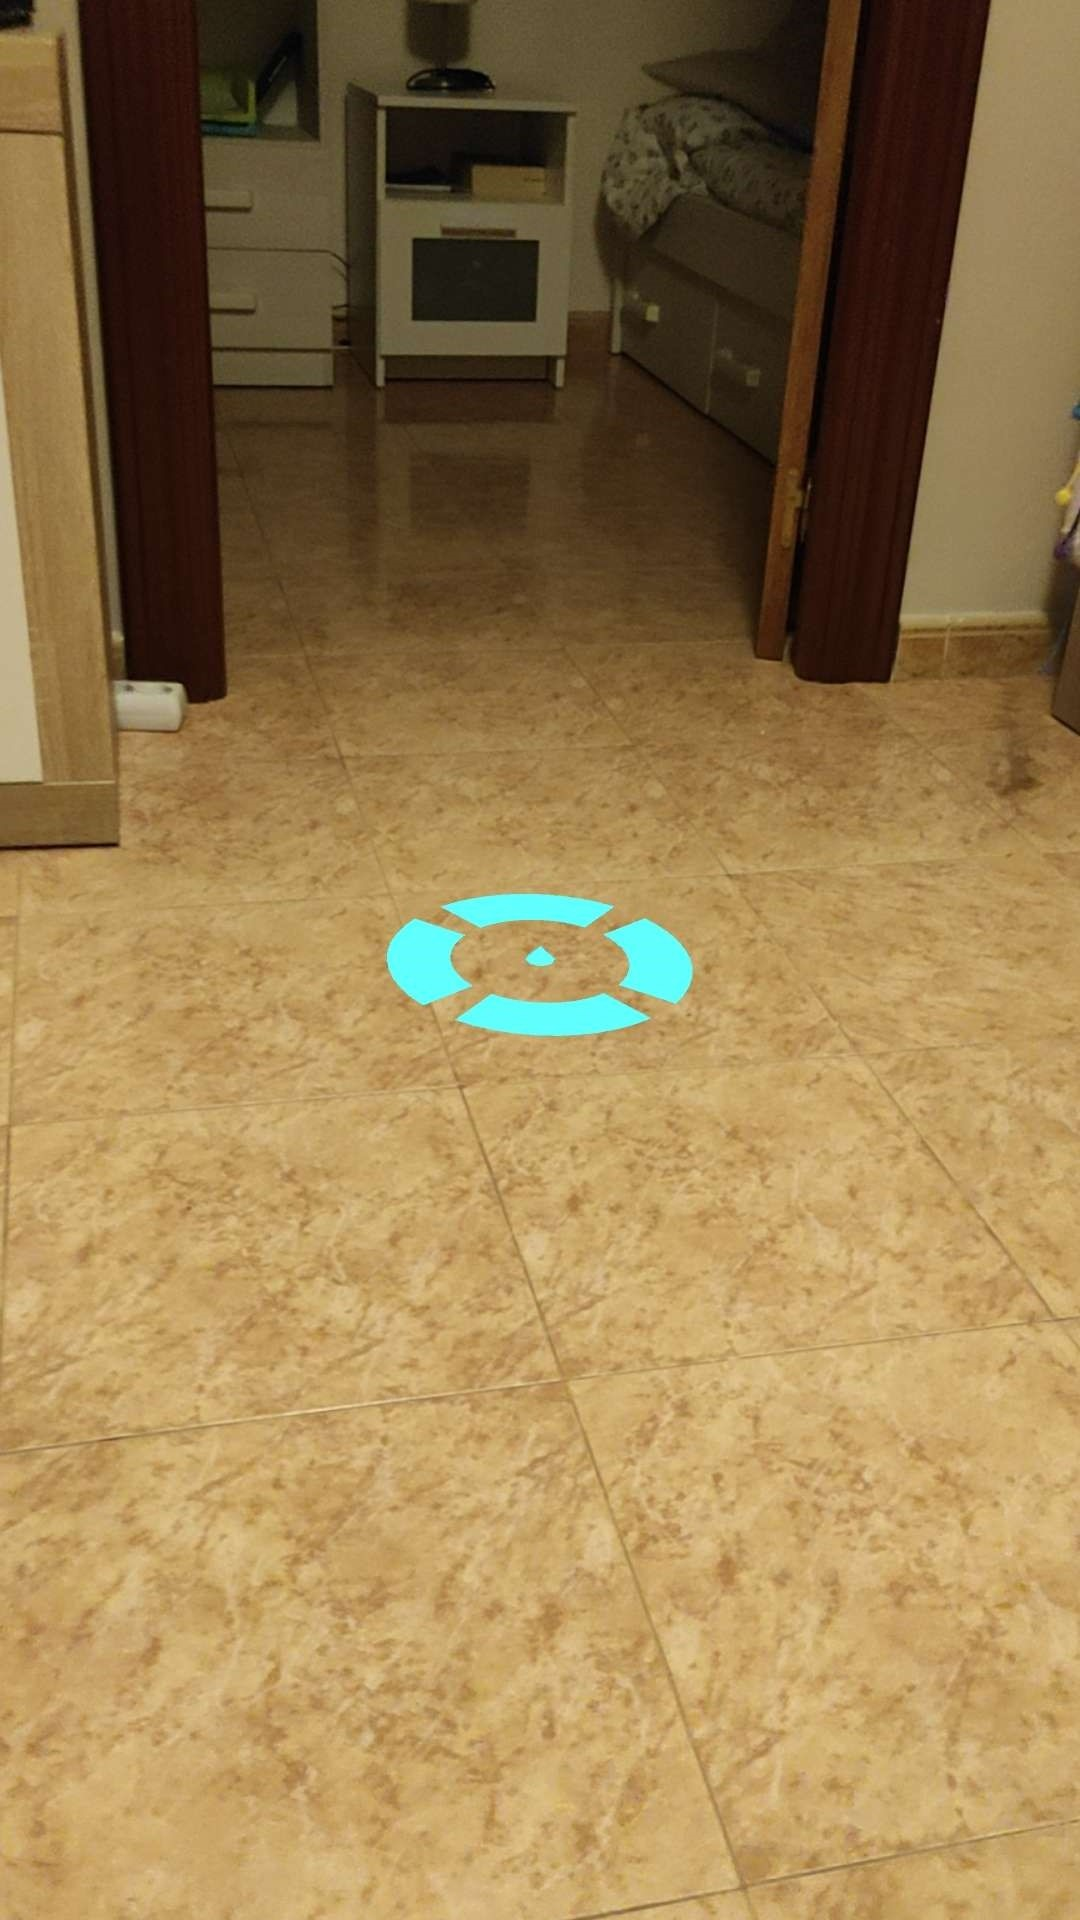
\includegraphics[width=0.2\textwidth]{3_reticle.jpg}
\caption{La aplicación muestra las imágenes de la cámara y coloca la retícula sobre la superficie detectada.}
\label{fig:3_reticle}
\end{figure}

        \paragraph{}
        Una vez el usuario conceda los permisos, la aplicación accederá a la cámara, donde utilizará las imágenes recibidas para calcular superficies (figura \ref{fig:3_reticle}). Una vez detecte una superficie horizontal, el sistema mostrará la retícula.

\begin{figure}[H]
\centering
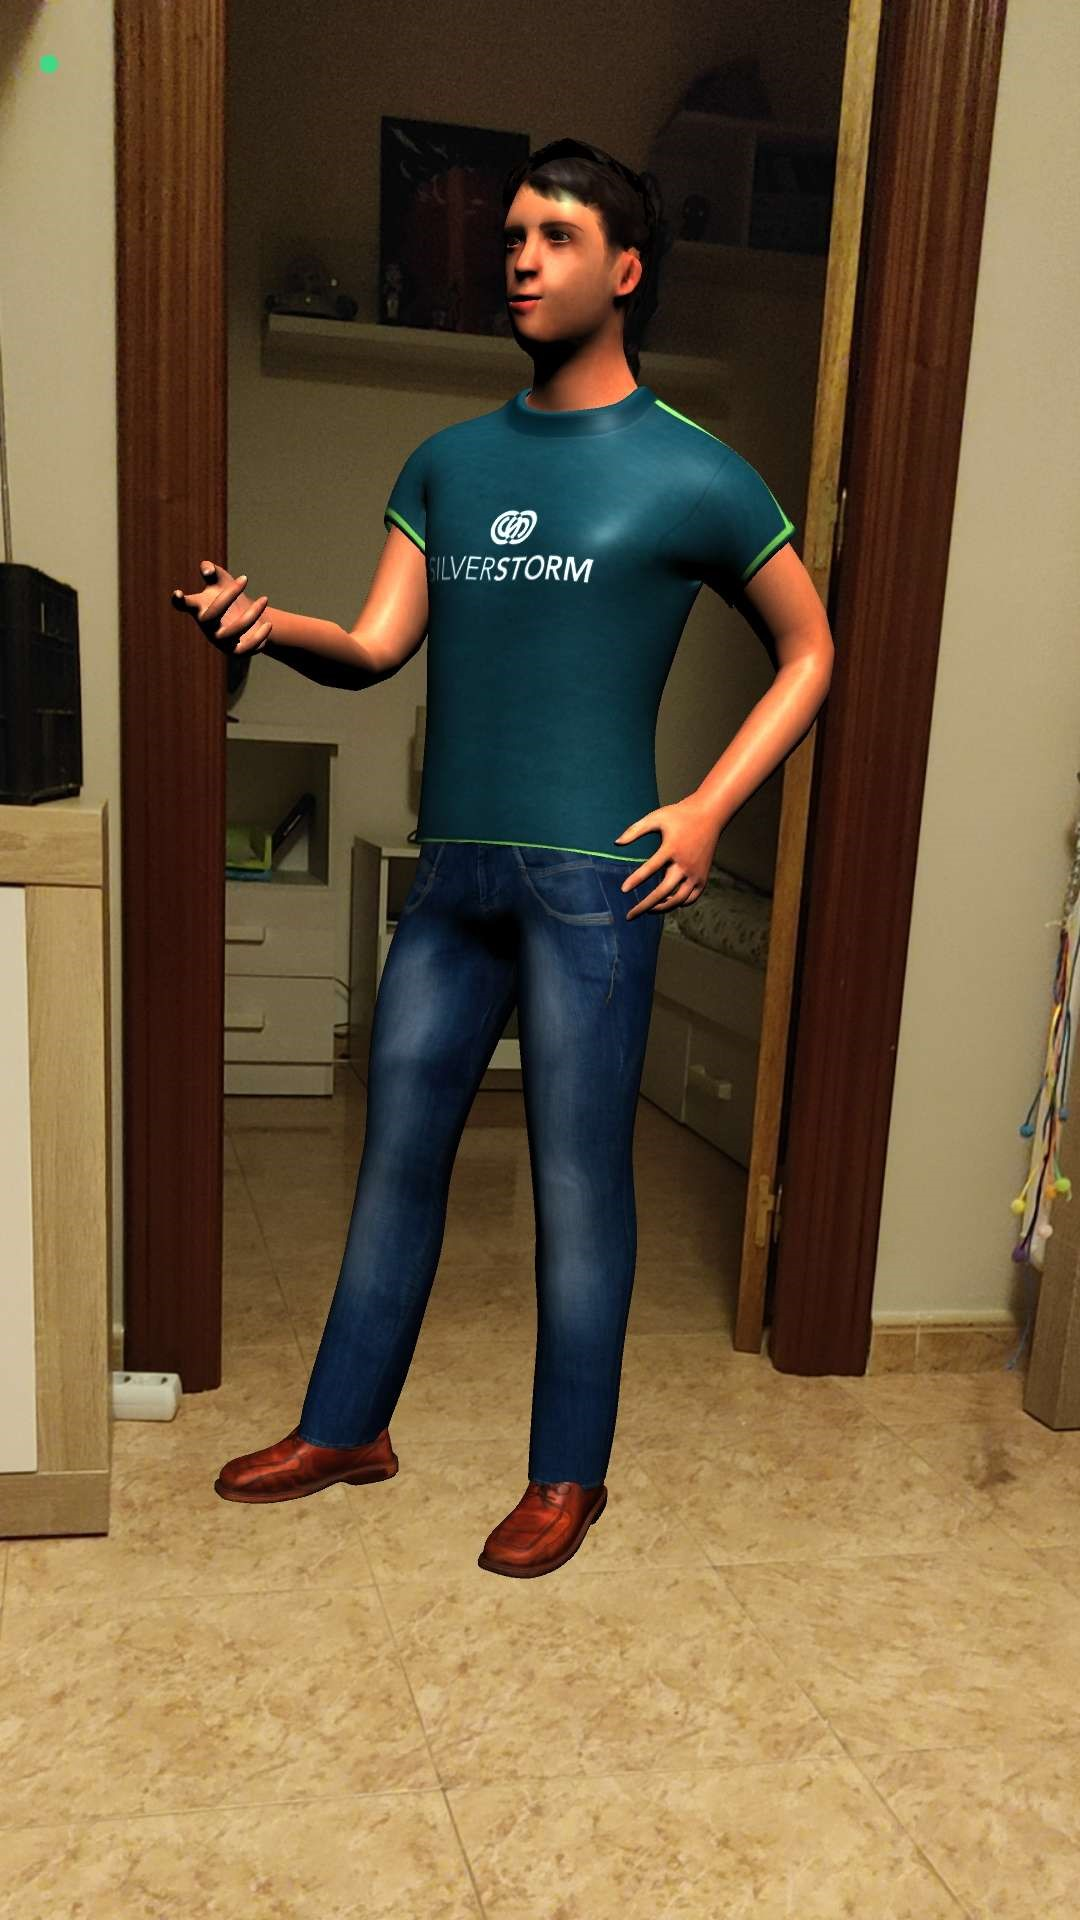
\includegraphics[width=0.2\textwidth]{4_model_appears.jpg}
\caption{Al pulsar sobre la pantalla, aparece el modelo y comienza su <<discurso>>.}
\label{fig:4_model_appears}
\end{figure}

        \paragraph{}
        Una vez se muestre la retícula, y no antes, el usuario podrá mostrar al modelo en 3D al pulsar sobre la pantalla, apareciendo allá donde estuviese la retícula (figura \ref{fig:4_model_appears}). Además, el modelo comenzará a hablar y moverse y la retícula desaparecerá al realizar esta acción. Su voz aumentará o disminuirá en relación a la distancia entre la cámara y el modelo, y el sonido se percibirá por los auriculares en relación a la posición del modelo con respecto a la cámara.

\begin{figure}[H]
\centering
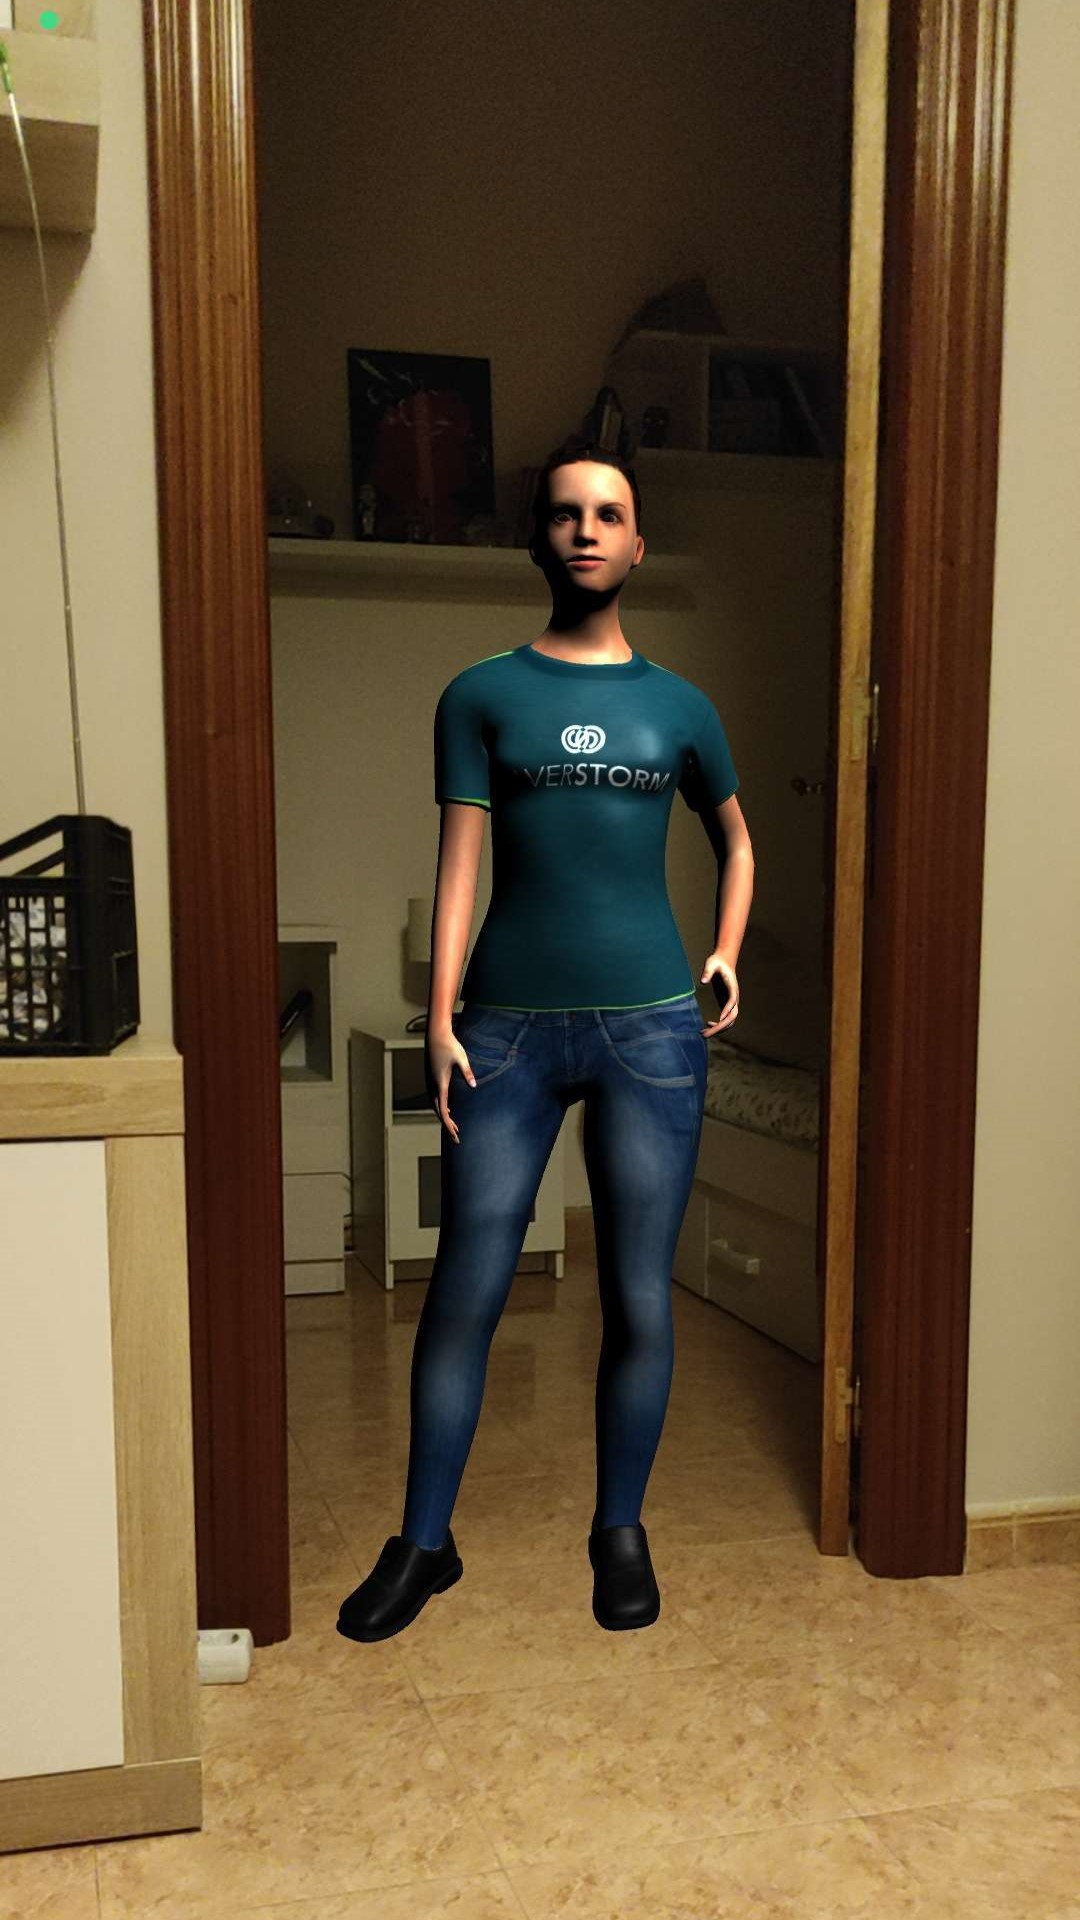
\includegraphics[width=0.2\textwidth]{5_alternate_model.jpg}
\caption{La selección del modelo es completamente aleatoria.}
\label{fig:5_alternate_model}
\end{figure}

        \paragraph{}
        El modelo utilizado se seleccionará de manera completamente aleatoria, pudiendo aparecer uno de dos diseños distintos (figura \ref{fig:5_alternate_model}). Cada uno tendrá su propia voz, aunque las animaciones son similares.

\begin{figure}[H]
\centering
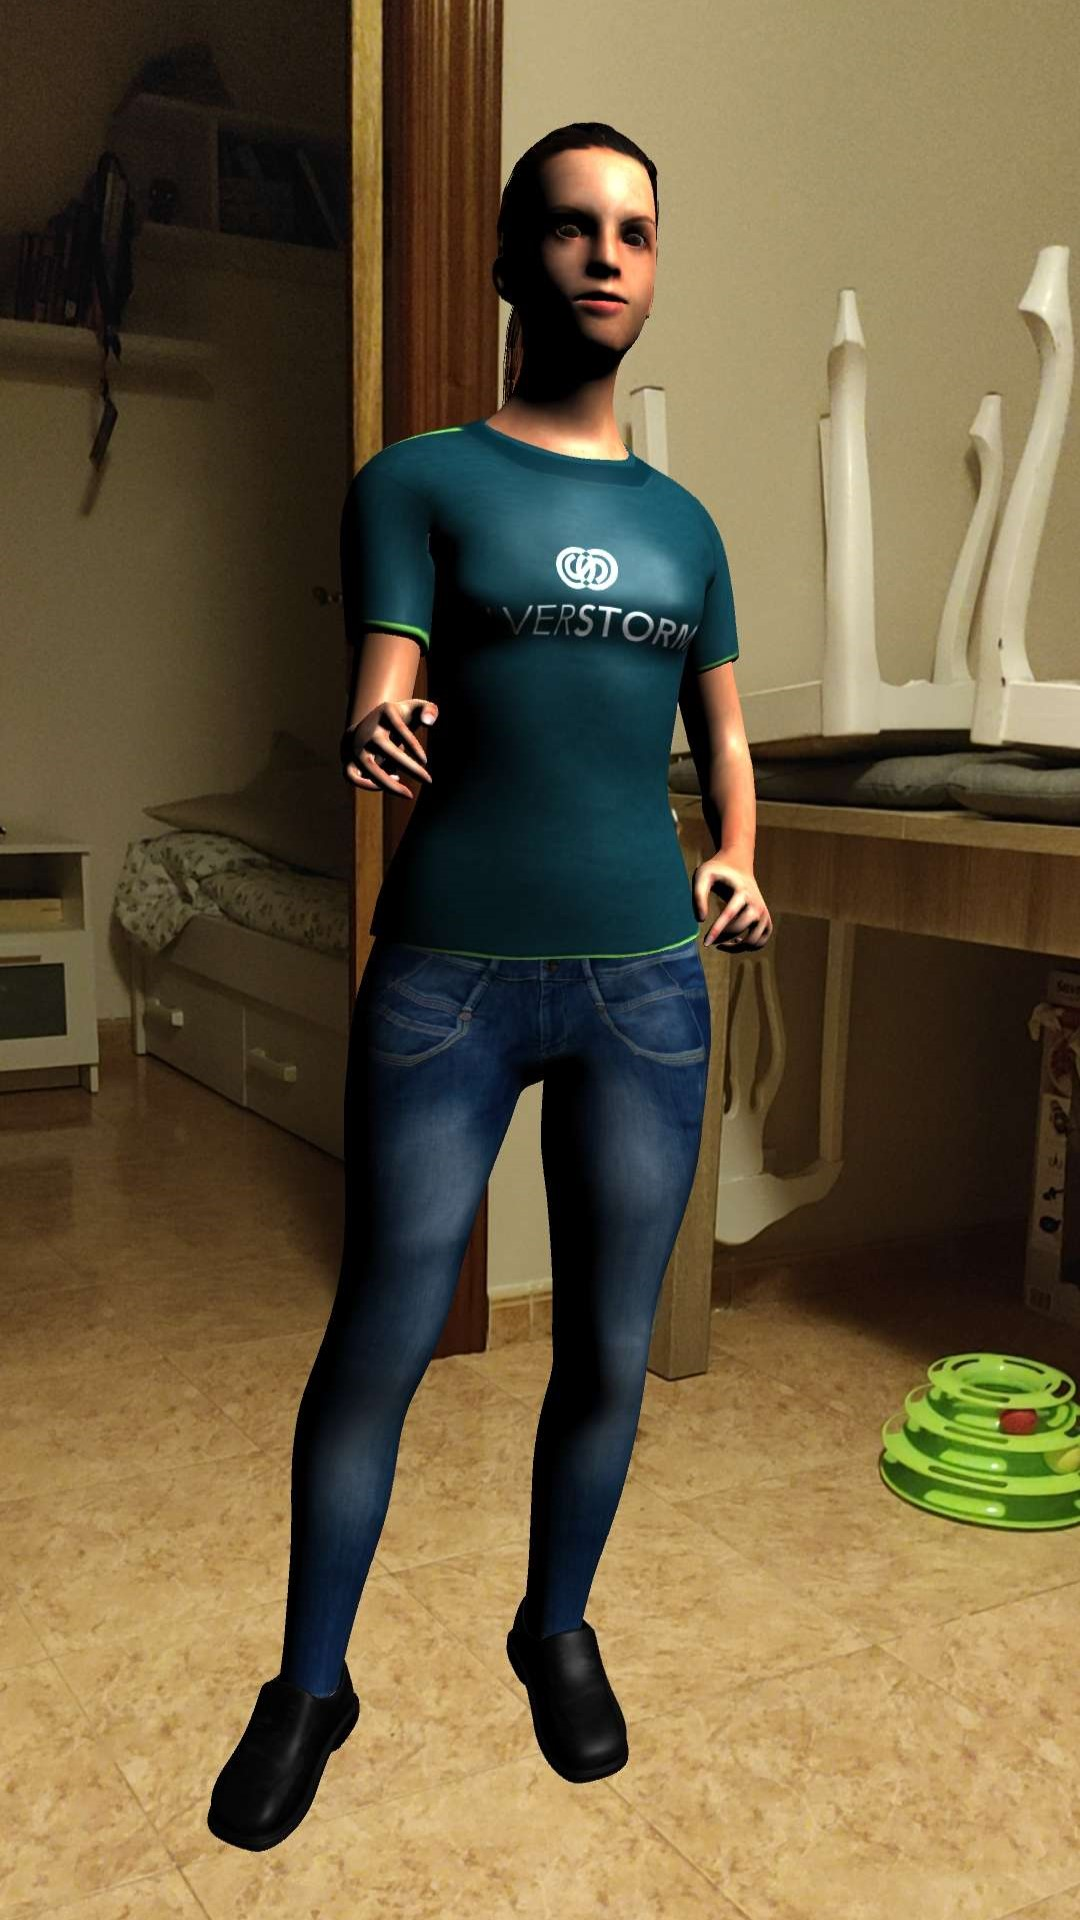
\includegraphics[width=0.2\textwidth]{6_moving_model.jpg}
\caption{El modelo podrá ser desplazado de lugar.}
\label{fig:6_moving_model}
\end{figure}

        \paragraph{}
        Una vez cargado el modelo y mostrado en la sesión, el usuario podrá volver a pulsar sobre la pantalla para mover al modelo, sin que esto interrumpa la animación o la voz del modelo (figura \ref{fig:6_moving_model}.

\begin{figure}[H]
\centering
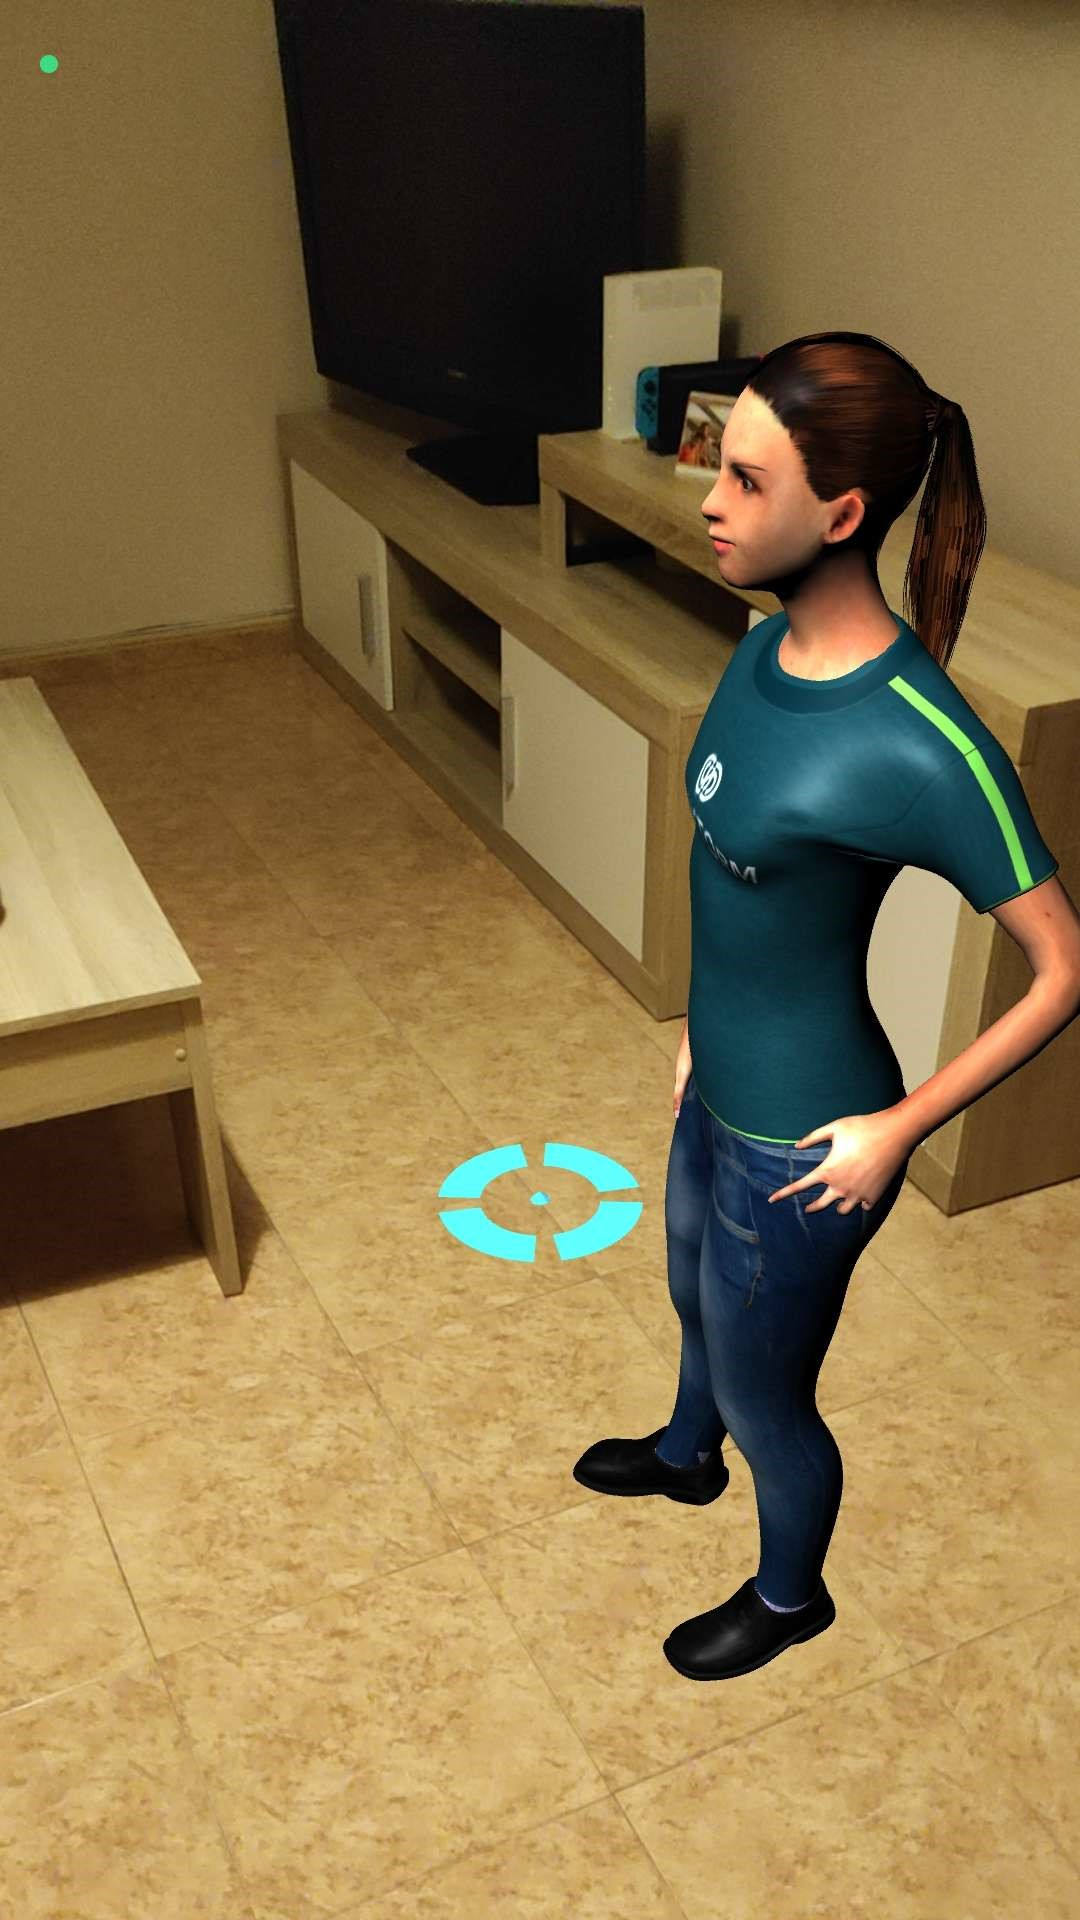
\includegraphics[width=0.2\textwidth]{7_end_of_animation.jpg}
\caption{La retícula vuelve a aparecer al terminar la animación.}
\label{fig:7_end_of_animation}
\end{figure}

        \paragraph{}
        Una vez termine la animación y el discurso volverá a aparecer la retícula, indicando al usuario que puede volver a pulsar sobre la pantalla para que vuelva a comenzar el discurso y la animación (figura \ref{fig:7_end_of_animation}. Para cerrar la sesión de \ra, el usuario podrá pulsar el botón de <<volver>> del móvil, con lo que, de manera previa, se finalizarán la animación y el audio.

\end{document}